\chapterimage{Fig/Chapter4/goutte_only_transparent.png}

\chapter{Experimental observation of k/-k correlations in the depletion of a weakly-interacting Bose gas}

\label{sec:chapter_4}

The Bogoliubov interacting Bose gas has been the subject of a large variety of experimental studies, both aiming at measuring the Bogoliubov spectrum of excitations \cite{fontaine2018,miller1962,ozeri2005,stepanov2019} as well as the quantum depletion \cite{chang2016,lopes2017,xu2006observation}. However, even though there have been some experimental work measuring the Lee, Huang and Yang beyond-mean field correction to the ground-state energy \cite{navon2010equation,skov2021observation}, an experimental study of the correlations in the many-body ground-state, and more precisely the observation of the \kmk pairs, is yet to be done more than 60 years after their prediction \cite{lee1957}. As we have seen through the different chapters of this thesis, our experimental setup is perfectly suited for such an investigation. 

We will present in this chapter the main result of this thesis, namely the observation of the \kmk pairs of the quantum depletion. We will detail the numerical procedure and the analysis method used to extract the correlation signals and present the experimental results. With the theoretical developments of Chapter \ref{sec:chapter_1}, we will show how we can link the measured anomalous correlation signal to the \kmk pairs of the quantum depletion by studying the effect of temperature, the widths and amplitudes of the correlation peak, as well as the fluctuations of the atom number difference between modes $\bm{k}$ and $-\bm{k}$. In addition, we will show how our measurement constitutes a first step towards showing the presence of momentum-space entanglement in many-body equilibrium states. We will finally discuss some preliminary results on the evolution of the correlation signals with the region of momentum space they are probed in.

\section{Numerical procedure to measure two-body correlations}

\label{sec:numerical_calculation}

As we have seen in the previous chapter, we are capable for each experimental run of reconstructing the 3D momentum coordinates of every atom detected by the $\He$ detector. We must now devise a numerical procedure to extract the two-body correlation signals from this raw data. Our goal is then to compute the general normalized second-order correlation function:

\begin{equation}
    g^{(2)} (\bm{k},\bm{k'}) = \frac{\mean{\hat{a}^{\dagger}_{\bm{k}} \hat{a}^{\dagger}_{\bm{k'}} \hat{a}_{\bm{k}} \hat{a}_{\bm{k'}}}}{\mean{\hat{a}^{\dagger}_{\bm{k}} \hat{a}_{\bm{k}}} \mean{\hat{a}^{\dagger}_{\bm{k'}} \hat{a}_{\bm{k'}} }}
\end{equation}

\noindent We recognize that $\mean{\hat{a}^{\dagger}_{\bm{k}} \hat{a}_{\bm{k}}}$ is the momentum density in mode $\bm{k}$ that we will write $\rho(\bm{k})$ in the following. We remind the result of Chapter \ref{sec:chapter_1} for weakly-interacting bosons that the $\gtwo$ function will take values different from 1 in two cases:

\begin{itemize}
    \item For $\bm{k'} \simeq \bm{k}$, the \textbf{normal} correlations corresponding to the Hanbury Brown and Twiss effect also known as bosonic bunching.
    \item For $\bm{k'} \simeq -\bm{k}$, the \textbf{anomalous} correlations signalling \kmk pairs in the quantum depletion.
\end{itemize}

In practice, plotting the $\gtwo$ function is not straightforward. On the one hand, the function here is 6D and thus hard to plot in an intelligible way. On the other hand, obtaining a sufficient signal to noise ratio for correlation measurements between single modes $\bm{k}$ and $\bm{k'}$ whose volume is typically $(1/L_{\rm{BEC}})^3$ is hardly possible. The idea is then to average the $\gtwo$ function over a large volume $\Omega_k$ of the momentum space and introduce a new parameter $\delta \bm{k}$ to write:

\begin{equation}
    g_{A}^{(2)} (\delta {\bm k})=\frac{\int_{\Omega_{k}} \langle \hat{a}^{\dagger}_{\bm k} \hat{a}^{\dagger}_{\delta {\bm k} - {\bm k}} \hat{a}_{\bm k} \hat{a}_{\delta {\bm k} - {\bm k}} \rangle \mathrm{d}{\bm k}}{\int_{\Omega_{k}} \rho(\bm k) \rho(\delta {\bm k} - {\bm k}) \mathrm{d}\bm{k}}
    \label{Eq:g2_anomalous}
\end{equation}

\begin{equation}
    g_{N}^{(2)} (\delta {\bm k})=\frac{\int_{\Omega_{k}} \langle \hat{a}^{\dagger}_{\bm k} \hat{a}^{\dagger}_{\delta {\bm k} + {\bm k}} \hat{a}_{\bm k} \hat{a}_{\delta {\bm k} + {\bm k}} \rangle \mathrm{d}{\bm k}}{\int_{\Omega_{k}} \rho(\bm k) \rho(\delta {\bm k} + {\bm k}) \mathrm{d}\bm{k}}
    \label{Eq:g2_normal}
\end{equation}

\noindent With this definition, we see that for $\delta \bm{k}=\bm{0}$, we are either looking at \textbf{anomalous} \kmk correlations (equation \ref{Eq:g2_anomalous}) or \textbf{normal} \kk correlations (equation \ref{Eq:g2_normal}). Note that the absence of a subscript $(N,A)$ in the following denotes a general calculation valid for both normal and anomalous correlation functions. We reduced the 6D function to a 3D function of the parameter $\delta \bm{k}$ which equals $\bm{0}$ when the correlation condition $\bm{k'} = \pm \bm{k}$ is fulfilled. This gives us a natural way to evaluate $\gtwo (\delta \bm{k})$ with the experimental data: we compute the values of the parameter $\delta \bm{k}$ for every detected atom pairs in an experimental run by calculating their momentum sum or difference for anomalous and normal correlations respectively. By computing the histogram of these values and averaging over many experimental runs, we evaluate the numerator of equation \ref{Eq:g2_anomalous} or \ref{Eq:g2_normal} respectively.

\subsection{Description of the algorithm}

The algorithm described here is similar to the one used in our previous works \cite{carcy2019momentum,cayla2020} and detailed in \cite{carcy_these,cayla_these}. This previous version was mainly designed for the observation of bosonic bunching. I adapted the algorithm to make it suitable for the calculation of \kmk correlations as well, as we will discuss now.

\subsubsection{Numerator calculation}

The first step is to compute the numerator of equations \ref{Eq:g2_anomalous} or \ref{Eq:g2_normal} that we denote $G^{(2)}(\delta \bm{k})$. We note $N_{\rm{runs}}$ the number of experimental runs and $N_{i}$ the number of atoms in the $i$-th shot. The procedure is as follows:

% \begin{algorithm}
% \caption{$G^{(2)}$ calculation}
%     \begin{algorithmic}{}
%         \FOR{$i=1:N_{runs}$}
%             \FOR{$j=1:N_{i}$}
%                 \STATE Compute $\vec{k}_i+\vec{k}_j$
%                 \STATE Increment histogram $G^{(2)}$ corresponding pixel
%             \ENDFOR
%         \ENDFOR
%     \end{algorithmic}{}
% \end{algorithm}


\begin{algorithm}[h!]
 \caption{$G^{(2)}$ calculation}
    \begin{algorithmic}
         \For{$i=1:N_{\rm{runs}}$}
            \For{$j=1:N_{i}$}
               \For{$p=1:N_{i}$}
                    \State Compute $\delta \bm{k} = \bm{k}_j \pm \bm{k}_p$
                    \State Increment the corresponding voxel in 3D histogram $G^{(2)}$ 
                \EndFor
            \EndFor
        \EndFor
\end{algorithmic}

\end{algorithm}

\noindent We end up with a 3D histogram where each voxel is associated to a value of $\delta \bm{k} = (\delta k_x,\delta k_y, \delta k_z)$ and records how many atom pairs have this specific momentum sum or difference, depending on the kind of the correlations probe. The voxels are set to be cubic of dimension $\Delta k_{\parallel}$. The value of $\Delta k_{\parallel}$ is adapted so that we can properly resolve the correlation peaks while ensuring a proper signal to noise ratio. In practice, we use $\Delta k_{\parallel}= 1.2 \times 10^{-2} \ k_d$ for \kmk correlations and $\Delta k_{\parallel}= 6 \times 10^{-3} \ k_d$ for \kk correlations as the correlation peak is narrower than the anomalous one (see \ref{sec:width_correlation_theo}).

The major difference with the previous version of the algorithm (see Appendix of \cite{carcy2019momentum}) is that we record here the full 3D histogram of calculated $\delta \bm{k}$ on every pair of atoms. The procedure was originally made simpler by calculating three one-dimensional histograms, one for each direction of space. Each of these histograms represents a one-dimensional cut of the general 3D correlation function $G^{(2)}(\delta \bm{k})$. For instance, to obtain the $x$ direction histogram, for the atom $j$ in run $i$, we calculate $\delta k_x$ only for atoms $p$ close enough in momentum space to find a \kk correlations, \ie with $|k_y^{(j)}-k_y^{(p)}| \leq \Delta k_{\perp}$ and $|k_z^{(j)}-k_z^{(p)}| \leq \Delta k_{\perp}$, where $\Delta k_{\perp}$ defines a transverse integration (see later). This method obviously saves computing time and RAM space, but is not suited to look for \kmk correlations.

At this point, we record in the central voxels associated to $\delta \bm{k} \simeq \bm{0}$ what we call \textbf{true coincidences}, namely two atoms detected conjointly as a result of \kmk pairing or bosonic bunching. However, we also record \textbf{accidental coincidences} that do not represent correlations but result from the momentum distribution of the atoms. We then need a normalization process to get rid of the contribution of accidental coincidences, \ie a method to compute the denominator of equation \ref{Eq:g2_anomalous} or \ref{Eq:g2_normal}.

\subsubsection{Denominator calculation}

\label{sec:algo}

We now compute the denominator of equation \ref{Eq:g2_anomalous} or \ref{Eq:g2_normal}, representing the effect of accidental coincidences. To perform this calculation, we would like to use a sample of uncorrelated atoms with the same momentum density than our experimental data. This can be done by merging all experimental shots together, each shot being uncorrelated with one another. We then apply the procedure we have just described to this data set. However, the correlations present within single shots remain in this large file. In the end, the total number of correlations in the numerator is $\sum_i N_i^2$ whereas the number of coincidences in the merged file is $(\sum_i N_i)^2$. With $\bar{N}$ the mean number of atoms per shot, we see that:

\begin{equation}
      \frac{\sum_i N_i^2}{(\sum_i N_i)^2}=\frac{N_{\rm{runs}} \bar{N}^2}{N_{\rm{runs}}^2 \bar{N}^2}=\frac{1}{N_{\rm{runs}}}
\end{equation}{}

\noindent Therefore, with enough shots, the contribution of residual coincidences is negligible and the normalization procedure valid. 

In the end, the integrated $g^{(2)}$ function is obtained by dividing the numerator histogram by the denominator and multiplying by the normalization factor $\frac{(\sum_i N_i)^2}{\sum_i N_i^2}$ that takes into account the number of coincidences of the numerator and denominator. Note that it is possible to take a fraction of all atoms for the denominator calculation to avoid large computation time. This is particularly handy to have quick first results before launching longer calculations for a nicer signal-to-noise ratio.



\subsection{Saturation of the detector and reconstruction errors}

As we have seen in \ref{sec:saturation_effect}, the algorithm reconstructing the positions at which the atoms fall on the MCP can give wrong results when the atomic flux is too high, which is typically the case with the very dense condensed diffraction peaks. This effect is particularly detrimental to the measurements described in this chapter as it artificially creates \kmk pairs. To circumvent this issue, we remove from the analysis the momentum region where $|k_z| < 0.05 \ k_d$ which corresponds to the region where the wrongly reconstructed BEC atoms are, at the expense of losing some possible ``true'' pairs located in this region. We check that the wrongly reconstructed atoms have been correctly removed from the analysis by watching the saturation cross disappear as illustrated on Fig.-\ref{fig:saturation_correction}.

\begin{figure}
    \centering
    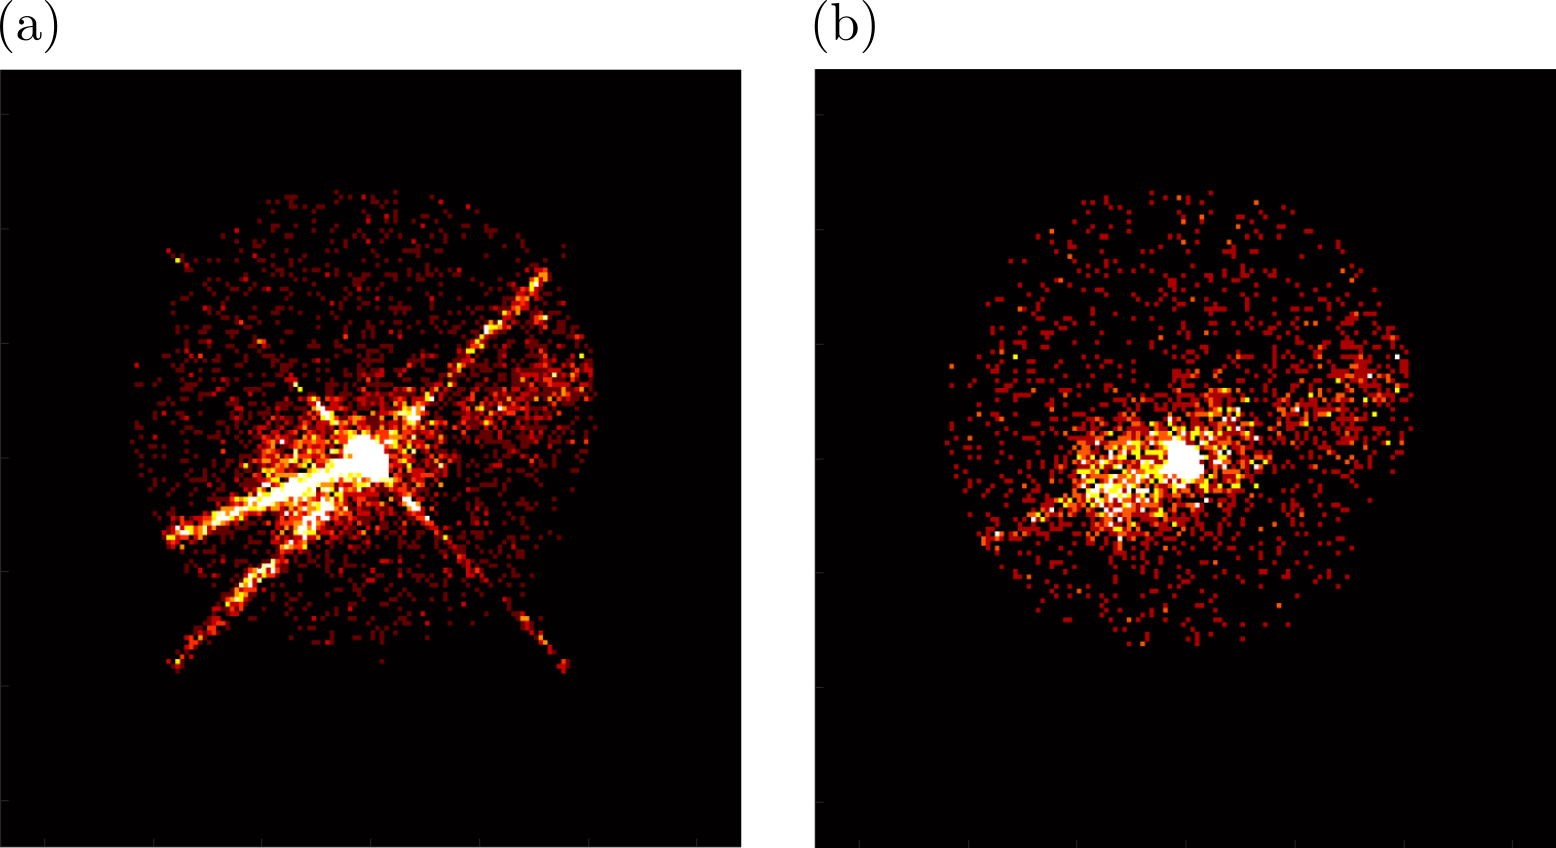
\includegraphics[width=\textwidth]{Fig/Chapter4/correction_saturation.png}
    \caption[Correction of software saturation]{Correction of software saturation. (a) Time integrated 2D MCP image, uncorrected, with the saturation cross. (b) Same image where the region $|k_z| < 0.05 \ k_d$ has been removed. The saturation cross has disappeared.}
    \label{fig:saturation_correction}
\end{figure}



\subsection{Transverse integration}

\label{sec:transverse_integration}

Now that we know how to numerically obtain the 3D histogram of the $\gtwo$ function, we must discuss how to represent the data. One of the most natural and intelligible way to do so is to plot 1D cuts of the $\gtwo$ function along the three direction of space to properly visualize the 3D correlation peak located in $\delta \bm{k} = \bm{0}$. To extract a 1D cut along the $x$ direction for instance, we could simply take the line of voxels verifying $\delta k_y=\delta k_z =0$. However, this is often not sufficient to have a proper signal-to-noise ratio. We therefore rather average the values of several voxels lines associated to $\delta \bm{k}$ values verifying $\abs{\delta k_y, \delta k_z} \leq \Delta k_{\perp}$ as illustrated on Fig-\ref{fig:cube_integration}, where $\Delta k_{\perp}$ defines the transverse integration. Note that this procedure applies for both normal and anomalous correlation functions.

\begin{figure}
    \centering
    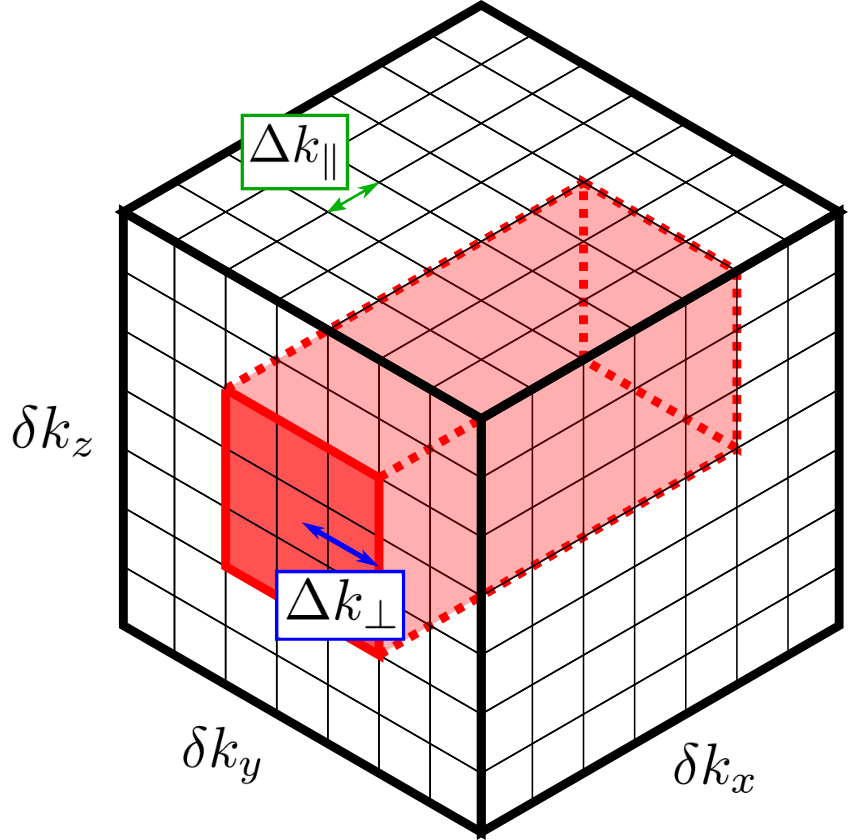
\includegraphics[width=0.45\textwidth]{Fig/Chapter4/cube_integration.png}
    \caption[Illustration of the transverse integration]{Illustration of the transverse integration. Every voxel contains the value of the $\gtwo$ function for a given value of $\delta \bm{k}=(\delta k_x, \delta k_y, \delta k_z$). The figure illustrates the procedure to take a 1D cut in the $x$ direction: we average over several pixel lines to increase the signal-to-noise ratio. This is the transverse integration $\Delta k_{\perp}$ as defined on the schematic.}
    \label{fig:cube_integration}
\end{figure}

We now write what is the signal that is plotted when this process is applied. The theoretical, normalized and integrated two-body correlation function is well modelled in first approximation by a 3D Gaussian function:

\begin{equation}
    \gtwo (\delta \bm{k}) = 1 + \eta_0 \prod_{i=x,y,z} \exp \left(\frac{-\delta k_i^2}{2 \sigma_i}\right)
    \label{eq:g2_theo}
\end{equation}

\noindent where we introduce $\eta_0$ the amplitude of the correlation peak and $\sigma_i$ the RMS width of the correlation peak in direction $i=x,y,z$. Importantly, we have assumed that the different correlation axis are separable. We re-write this equation to account for the transverse integration process, with the example of a cut along the $x$ direction:

\begin{equation}
    g^{(2)} \left(\delta k_{x}\right)=\frac{1}{\left(2 \Delta k_{\perp}\right)^{2}} \iint_{-\Delta k_{\perp}}^{\Delta k_{\perp}} \left( 1+ \eta_0 \prod_{i=x, y, z} \exp \left(\frac{-\delta k_{i}^{2}}{2 \sigma_i^{2}}\right) \mathrm{d} \delta k_y \mathrm{d} \delta k_z \right)
\end{equation}

\noindent This expression can be analytically evaluated and writes:

\begin{equation}
    g^{(2)} \left(\delta k_{x}\right)=1+\eta_0 \frac{2 \pi \sigma_y \sigma_z}{\left(2 \Delta k_{\perp}\right)^{2}} \exp \left(\frac{-\delta k_{x}^{2}}{2 \sigma_{z}^{2}}\right) \operatorname{erf}\left(\frac{\Delta k_{\perp}}{\sqrt{2} \sigma_{y}}\right) \operatorname{erf}\left(\frac{\Delta k_{\perp}}{\sqrt{2} \sigma_{z}}\right)
\end{equation}

Note that we have here neglected the small longitudinal integration induced by the size of the voxel, which is typically 3 times smaller than the RMS width of the correlation peaks in our experimental data. In addition, we assume that the correlation peaks are isotropic as the lattice potential and then the spatial size of the gas are isotropic, giving $\sigma_x=\sigma_y=\sigma_z=\sigma$. We thus see that when measuring any correlation peak amplitude with a Gaussian fit on a 1D cut of the $\gtwo$ function, we get a reduced amplitude $\eta$ that writes:

\begin{equation}
    \eta (\Delta k_{\perp})= \eta_{0} \times \frac{2 \pi \sigma^2}{(2\Delta k_{\perp})^2}\left[\rm{erf} \left(\frac{\Delta k_{\perp}}{\sqrt{2}\sigma} \right)\right]^2
    \label{eq:fit_integration}
\end{equation}

The idea is then to measure $\eta$ for several values of $\Delta k_{\perp}$ and fit the data with equation \ref{eq:fit_integration} with $\eta_0$ and $\sigma$ as free parameters. This is illustrated on Fig-\ref{fig:integration_kk} and Fig.-\ref{fig:eta_vs_int_kmk} for \kmk and \kk correlations respectively. For a single value of the transverse integration, $\eta$ is obtained by averaging the 3 amplitudes fitted on the 1D cuts along the 3 directions of space. The uncertainty on the parameters of the fit defines the error bars on the amplitude.

In addition, we have checked that the transverse integration process does not significantly change the width of the correlation peak as shown on the inset of Fig.-\ref{fig:eta_vs_int_kmk}. The extracted width is therefore the fitted width at the lowest transverse integration for which we get a satisfactory signal to noise ratio.

\begin{figure}
    \centering
    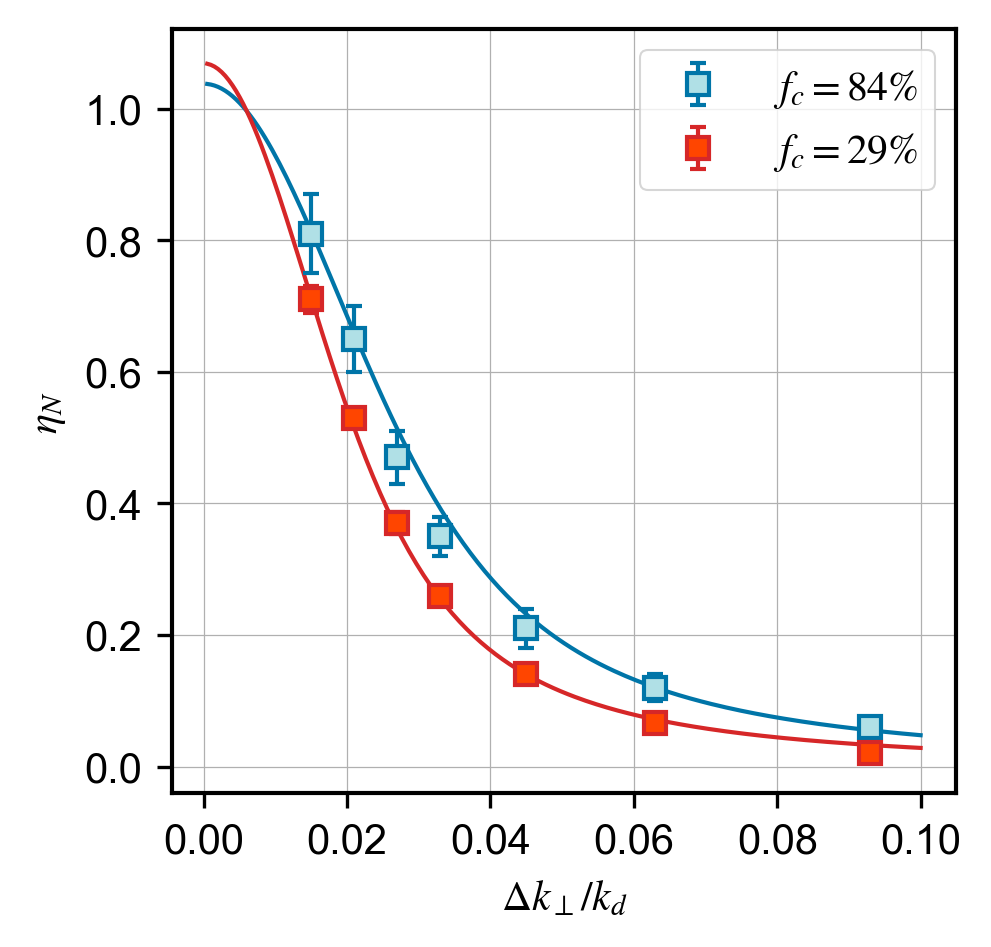
\includegraphics[width=0.65\textwidth]{Fig/Chapter4/eta_vs_int_kk.png}
    \caption[Fitted amplitude of the normal correlation peak $\eta_N$ as a function of the transverse integration $\Delta k_{\perp}$]{Fitted amplitude of the normal correlation peak $\eta_N$ as a function of the transverse integration $\Delta k_{\perp}$ for data sets with different condensed fraction. The data is fitted with model defined in equation \ref{eq:fit_integration} with $\eta_0$ and $\sigma$ as free parameters. This method allows us to extract the amplitude at zero transverse integration $\eta_{0,N}$.}
    \label{fig:integration_kk}
\end{figure}

\begin{figure}
    \centering
    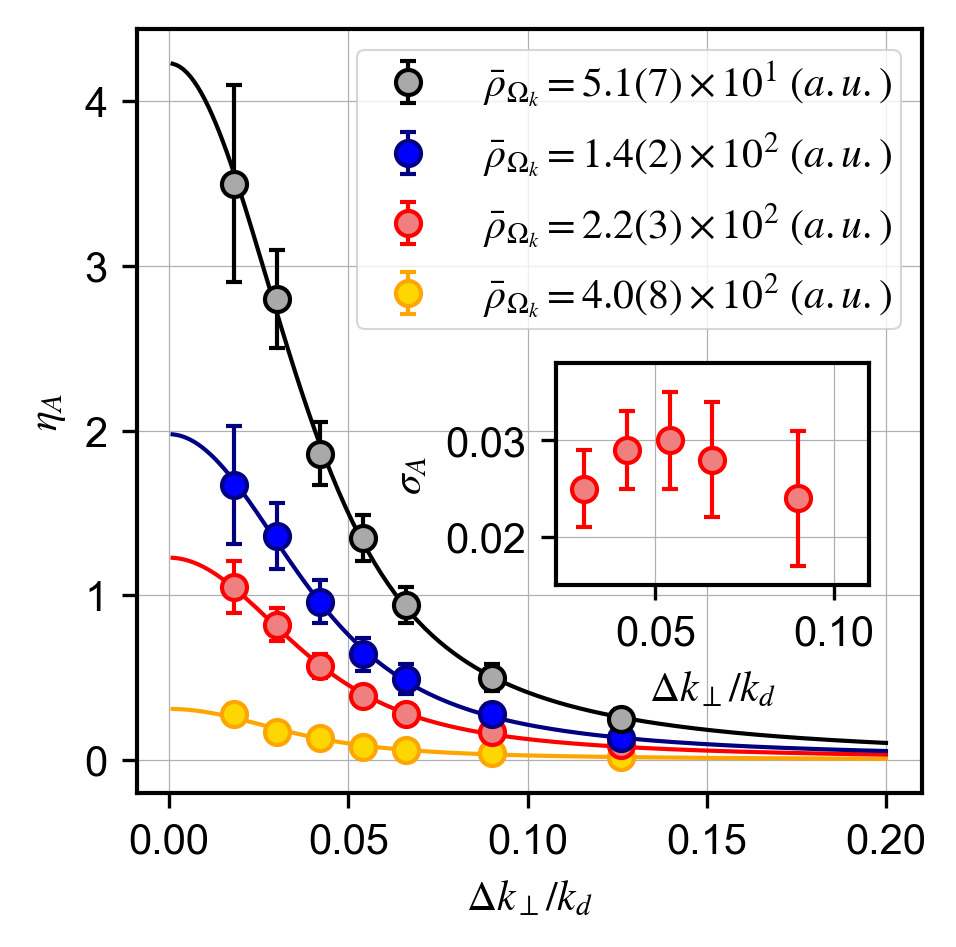
\includegraphics[width=0.65\textwidth]{Fig/Chapter4/eta_vs_int_kmk.png}
    \caption[Fitted amplitude of the anomalous correlation peak $\eta_A$ as a function of the transverse integration $\Delta k_{\perp}$]{Fitted amplitude of the anomalous correlation peak $\eta_A$ as a function of the transverse integration $\Delta k_{\perp}$ for data sets with various average densities $\rhob$ (see later). The inset represents the fitted width $\sigma_A$ as a function of the transverse integration $\Delta k_{\perp}$. No significant effect can be observed within the error bars.}
    \label{fig:eta_vs_int_kmk}
\end{figure}


\section{Observation of the pair correlation signal}

Now that we have determined the correct numerical procedure to extract the correlation signals from the raw data, we look to apply it on our experimental data. In this section, we will present the measured \kmk correlation signal of we which we will try to understand the main features. Our goal is to first identify clear arguments linking this signal to the quantum depletion, before going into quantitative details that will be the subject of the next section.

\subsection{Accessing the BEC depletion}
\label{sec:accessing_depletion}

In order to detect \kmk pairs in the depletion, it is absolutely crucial to remove from the analysis all atoms belonging to the BEC and its diffracted copies as explained in Chapter \ref{sec:chapter_1}. For each recorded data set and before running the algorithm, we remove all atoms outside the volume $\Omega_k$ that we design to exclude momentum regions with condensed atoms as illustrated on Fig-\ref{fig:omega_k}. We set $\Omega_k$ to have a cubic symmetry that matches the symmetry of the momentum distribution in a cubic lattice. We remove all atoms with $|k_i| < k_{\rm{min}}$ and $|k_i| > k_{\rm{max}}$ where $k_i$ is the momentum projection along an axis $i=x,y,z$. We use $k_{\rm{min}}=0.15 \, k_d$, corresponding to $\sim 6$ times the RMS width of the BEC peaks, in order to ensure that all condensed atoms have been removed. The high limit is set to $k_{\rm{max}}=0.85 \, k_d$ to exclude higher order peaks and is slightly smaller than the momentum range probed by the MCP. In terms of healing length, this corresponds to $0.85 \leq | k | \xi \leq 1.15$, \ie the region where the phononic character of the Bogoliubov quasi-particles is negligible and thus where finite temperature excitations do not contribute to the anomalous correlations. 

\begin{figure}
    \centering
    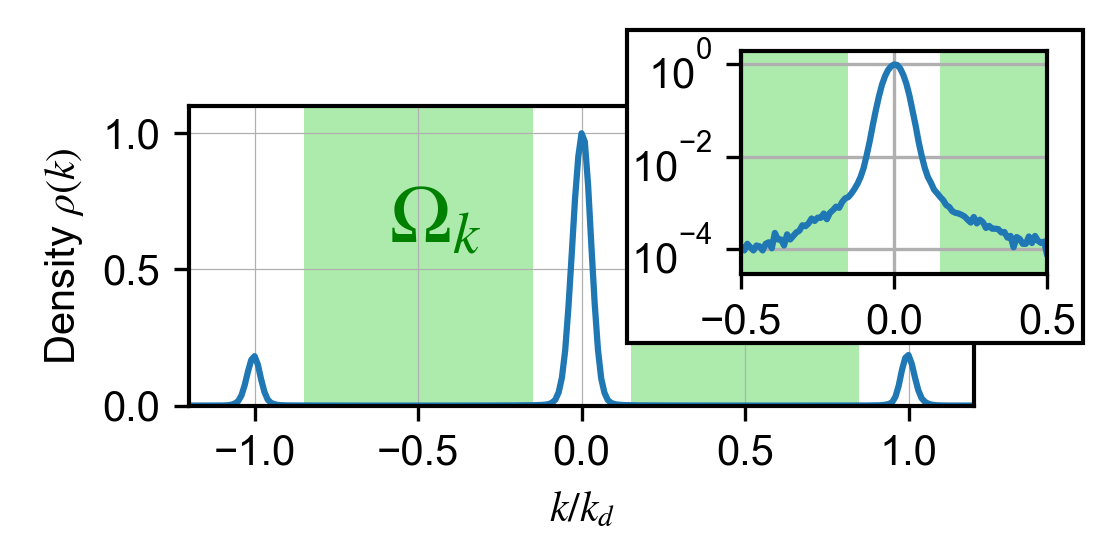
\includegraphics[width=0.8\textwidth]{Fig/Chapter4/densite.png}
    \caption[1D cut of the momentum density illustrating the integration volume $\Omega_k$]{1D cut of the momentum density illustrating the integration volume $\Omega_k$. The central peak corresponds to the BEC and the lateral peaks at $\pm \ k_d$ to diffraction peaks induced by the presence of the optical lattice. The green area shows the volume $\Omega_k$ containing the depleted atoms selected for the correlation measurement. While barely visible in linear scale, they can be seen in the log scale plot shown in inset.}
    \label{fig:omega_k}
\end{figure}

\subsection{Benchmarking of the algorithm with two-body collision spheres}

\label{sec:benchmark_algo}

Before using the algorithm to look for \kmk pairing signal in the depletion of a weakly-interacting Bose gas, it was crucial to test it on a data set with a large number of \kmk pairs to certify that it was working properly. Luckily, we could re-use the data taken for measuring two-body collisions during the time-of flight described in Chapter \ref{sec:chapter_3}. Indeed, because of the elastic character of the collision, every atom on a collision sphere is correlated with a partner on the other side of the sphere, yielding \kmk correlations in the reference frame of the center of mass of the colliding BECs \cite{hodgman2017solving,perrin2007observation}. In addition to the 3D diffraction data that we already presented, we also took data with a single lattice beam to induce 1D diffraction and obtain only two collision spheres (see Fig.-\ref{fig:1D_spheres}). The advantage is that we have a large number of atoms in these collision spheres, making the analysis easier. 

\begin{figure}
    \centering
    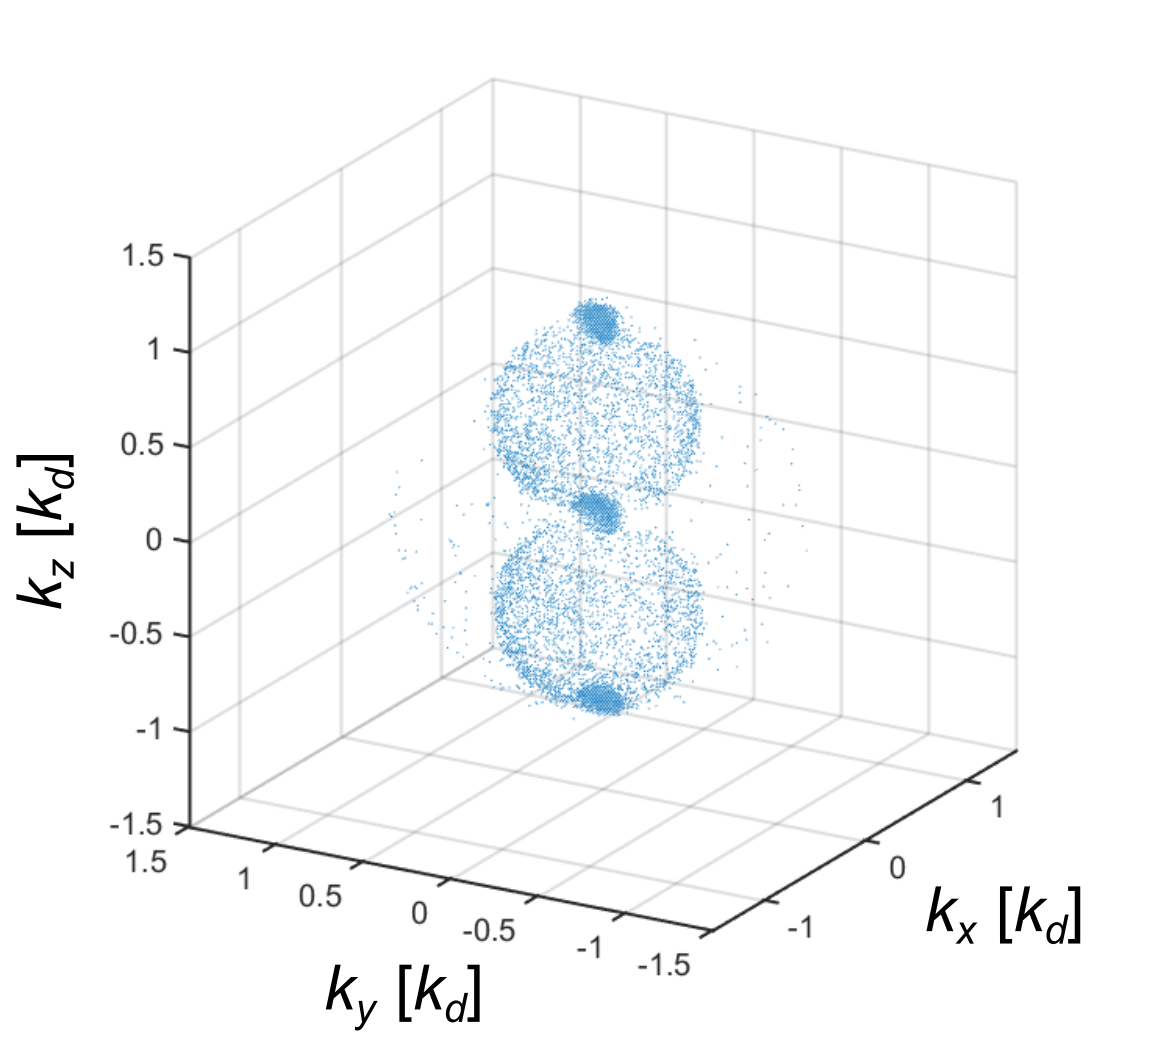
\includegraphics[width=0.7\textwidth]{Fig/Chapter4/1d_spheres.png}
    \caption[1D diffraction and associated collision spheres]{1D diffraction and associated collision spheres. Note that while the condensed peaks are shown here, they are removed before calculating the correlations.}
    \label{fig:1D_spheres}
\end{figure}

Contrary to the \kmk correlations of the quantum depletion, we de not expect a correlation peak at $\delta \bm{k}=\bm{0}$. If we consider for instance collisions between the 0th and 1st orders of diffraction along $z$, the overall momentum before and after the collision is $k_d \bm{z}$ ($\bm{z}$ is the unitary vector of the $z$ axis), so that the sum of the momenta of the two correlated atoms after the collision must be $k_d \bm{z}$. We thus expect a correlation peak for each sphere, one at $\delta k = (0,0,+1 \ k_d)$  and one at $\delta k = (0,0,-1 \ k_d)$.

We run the algorithm on the experimental data and obtain the results shown in Fig.-\ref{fig:kmk_kapitza}. We observe two correlations peaks at the expected locations! We can now extract the width and amplitude of the peaks with a Gaussian fit and see if they match with the results of \cite{tenart2020two} detailled in Chapter \ref{sec:chapter_3}. We find RMS widths of $\sigma_A^{(-1)}=2.3(9) \times 10^{-2} \ k_d$ and $\sigma_A^{(+1)}=2.7(8) \times 10^{-2} \ k_d$, the error bars being given by the uncertainty on the fit coefficients. This is consistent with the measured widths of the scattering halos presented in \ref{sec:width_halos}, namely $\delta k_s = 2.1(9) \times 10^{-2}$ for $\NBEC=1.25 \times 10^5$ close to the total number of atoms used here. 
The prediction of the amplitude is rather easy in this configuration as we know that every atom on the sphere has a momentum correlated partner, allowing us to compare it to the experiment. To count the experimental number of detected pairs, we use the following procedure:


\begin{enumerate}
    \item The voxel size is increased to $\Delta k_{\parallel} = 0.25 \ k_d$ so that a single voxel contains the correlation peak entirely to count all true correlations.
    
    \item We count the number of coincidences $N_{\rm{numerator}}$ in the central voxel of the numerator histogram of equation \ref{Eq:g2_anomalous}. 
 
   
    \item  We count the number of coincidences $N_{\rm{denominator}}$ in the central voxel of the denominator of equation \ref{Eq:g2_anomalous} to evaluate the number of accidental coincidences. 
    
    
    \item As the numerator contains both true and accidental coincidences, we evalute the number of true coincidences by subtracting the number of accidental coincidences and taking into account the normalization factor:
    \begin{equation}
          2N_{\rm{pairs}}=N_{\rm{numerator}} - N_{\rm{denominator}} \times \frac{\sum_i N_i^2}{(\sum_i N_i)^2}
    \end{equation}
    where the factor 2 is added as we define $N_{\rm{pairs}}$ as the number of pairs and we rather obtain the number of paired atoms with this formula.
  
\end{enumerate}

We find that the average number of detected pairs per run is $N_{\rm{pairs}}/N_{\rm{runs}}=6.25$. This number must be compared to the number of pairs that we expect from the number of atoms in the spheres that we evaluate using the following procedure:

\begin{itemize}
    \item Writing $N_{\rm{tot}}$ the total atom number in a given sphere, we know that we should detect $N_{\rm{tot}} \alpha_{\rm{MCP}}^2$ correlated atoms, where $\alpha_{\rm{MCP}}$ is the detection efficiency of the $\He$ detector. 
    \item The number of detected atoms in the considered sphere is simply $N_{\rm{tot}} \alpha_{\rm{MCP}}$ and accessible experimentally. Multiplying this number by $\alpha_{\rm{MCP}}$, we thus obtain the expected number of correlated atoms.
\end{itemize}

We find that we expect to detect $8.5(5)$ pairs per run which is rather consistent with the number of detected pairs per run. The uncertainty is given by the uncertainty on the detection efficiency. Note that as this experiment was done before the implemention the two-photon Raman transfer scheme, the detection efficiency was lower than what was calibrated in Chapter \ref{sec:chapter_3} and was equal to $\alpha_{\rm{MCP}}=6.5(4) \%$.




\begin{figure}
    \centering
    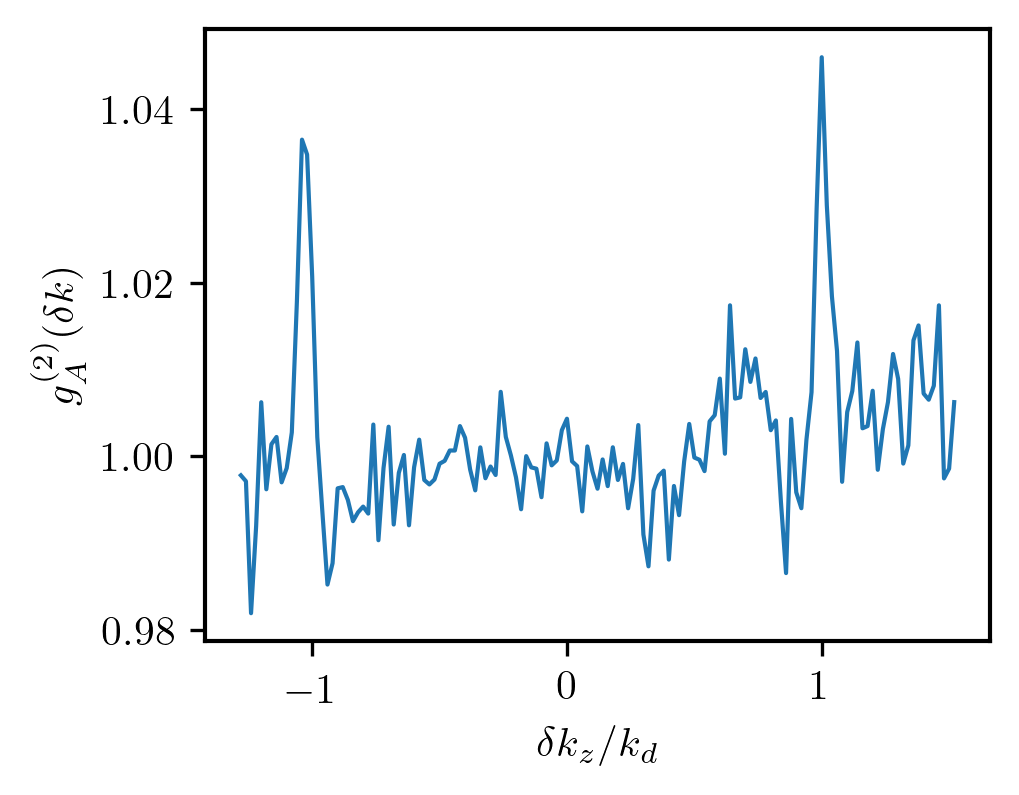
\includegraphics[width=0.7\textwidth]{Fig/Chapter4/kmk_kapitza.png}
    \caption[1D cut of the anomalous correlation function $\gtwo_A$ along the $z$ axis]{\NOTE{corriger décalage} 1D cut of the anomalous correlation function $\gtwo_A$ along the $z$ axis. We observe two correlation peaks, one for each correlation sphere. The peaks are not exactly at $-1 \ k_d$ and $+1 \ k_d$ due to a slight mis-recentering of the data. The longitudinal size of the voxels is $\Delta k_{\parallel}= 2 \times 10^{-2}$ and the transverse integration $\Delta k_{\perp}= 9 \times 10^{-2}$.}
    \label{fig:kmk_kapitza}
\end{figure}


\subsection{First characterization of the pair correlation signal}

\label{sec:post_selec}

As we have checked that the algorithm is working properly, we now look to observe the \kmk pairs of the quantum depletion.



\begin{figure}[]
    \centering
    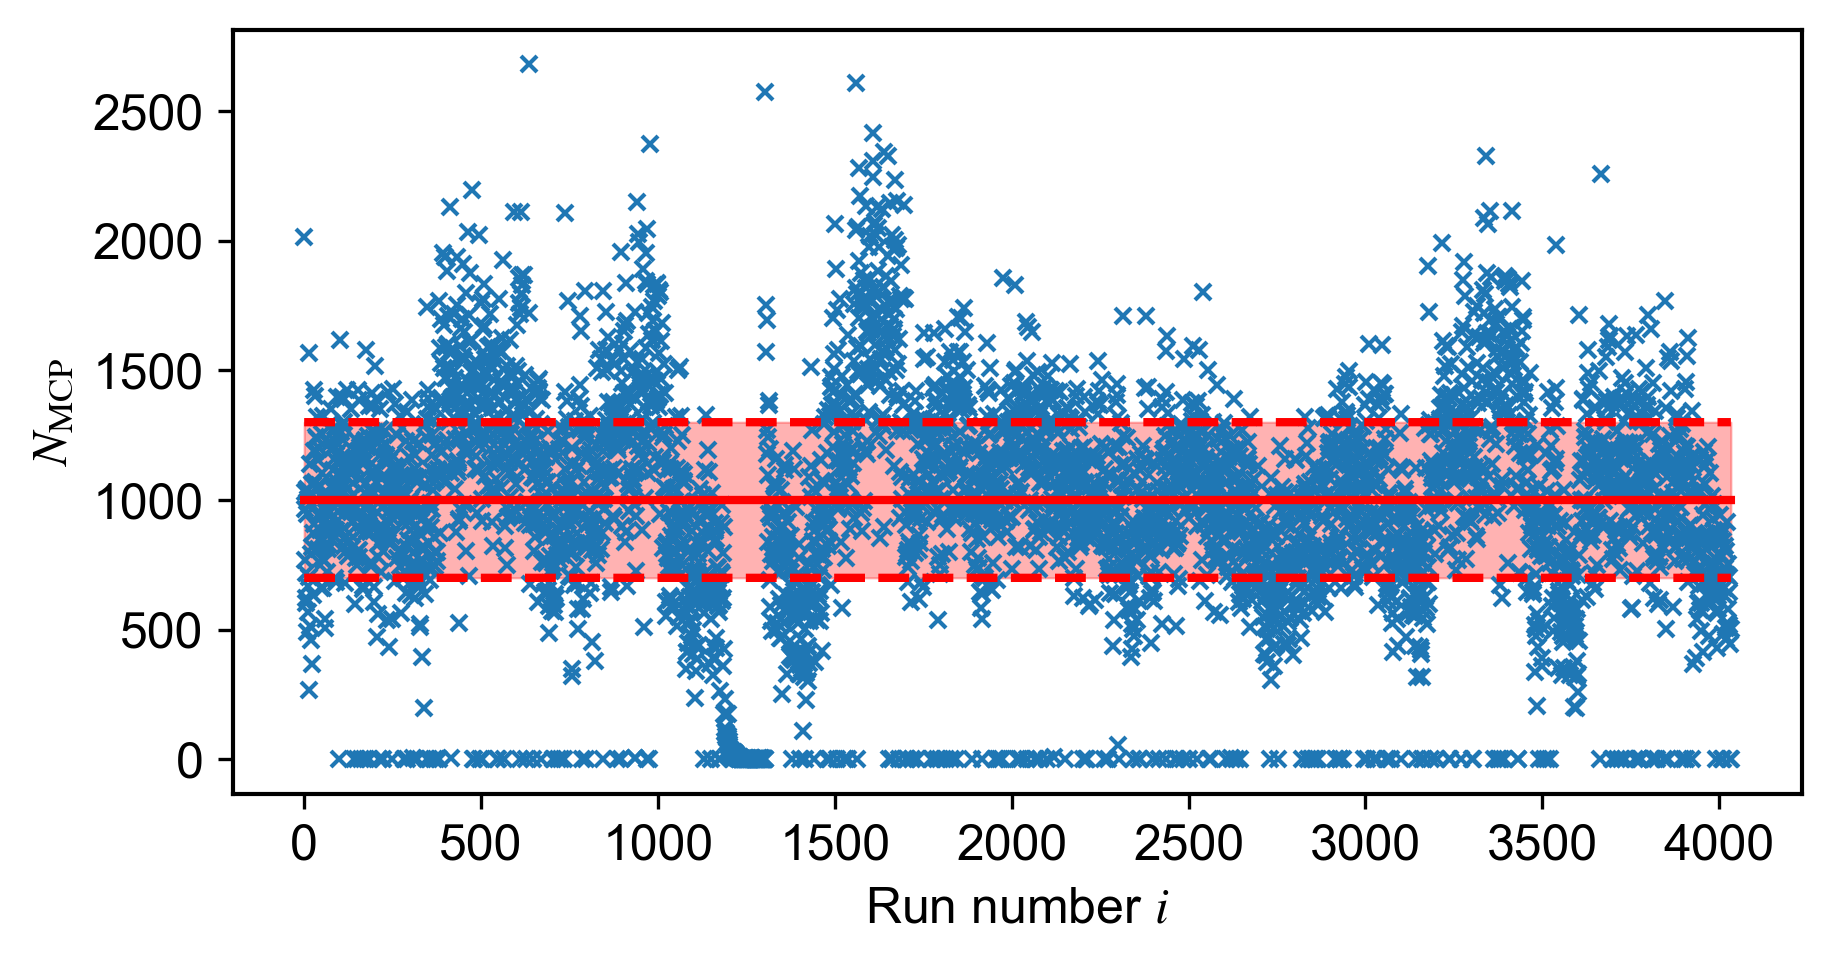
\includegraphics[width=0.95\textwidth]{Fig/Chapter4/n_fluctuations.png}
    \caption[Number of detected atoms $N_{\mathrm{MCP}}$ for each experimental runs of a data set]{Number of detected atoms $N_{\mathrm{MCP}}$ for each experimental runs of a data set. The full red line represents the target detected atom number. The red shaded area between the dashed lines illustrate the allowed fluctuations of the detected atom number. All runs outside of the red area are rejected.}
    \label{fig:n_fluctuations}
\end{figure}

We prepare a BEC with a target number of $\NBEC=5 \times 10^3$ atoms in an optical lattice of amplitude $V=7.75 \ E_r$. With this lattice amplitude, we are in the superfluid domain of the phase diagram in which we expect the \kmk correlations: we measure a condensed fraction of $84 \%$ corresponding to depletion level for which the Bogoliubov theory is expected to hold (see Supp. Mat. of \cite{lopes2017} \NOTE{check}). In order to have sufficient statistics, we repeat the experiment $\sim 4,000$ times. In practice, we cannot prepare BECs with the exact same number of atoms at each shot. We then need to post-select the data and remove runs with a detected atom number falling too far from the target number. This is one of the strengths of our experiment: as each atom has the same probability of being detected, we can select shots with the good total atom number a posteriori with a precision unattainable with optical imaging measuring densities. This must however be mitigated by the fact saturation effects reduces the number of detected atoms in a way that can be hard to predict precisely. We allow for $30 \%$ fluctuations around the target number (see Fig.-\ref{fig:n_fluctuations}) and end up conserving around $\sim 2,000$ runs on which we run the algorithm.

\begin{figure}[ht!]
    \centering
    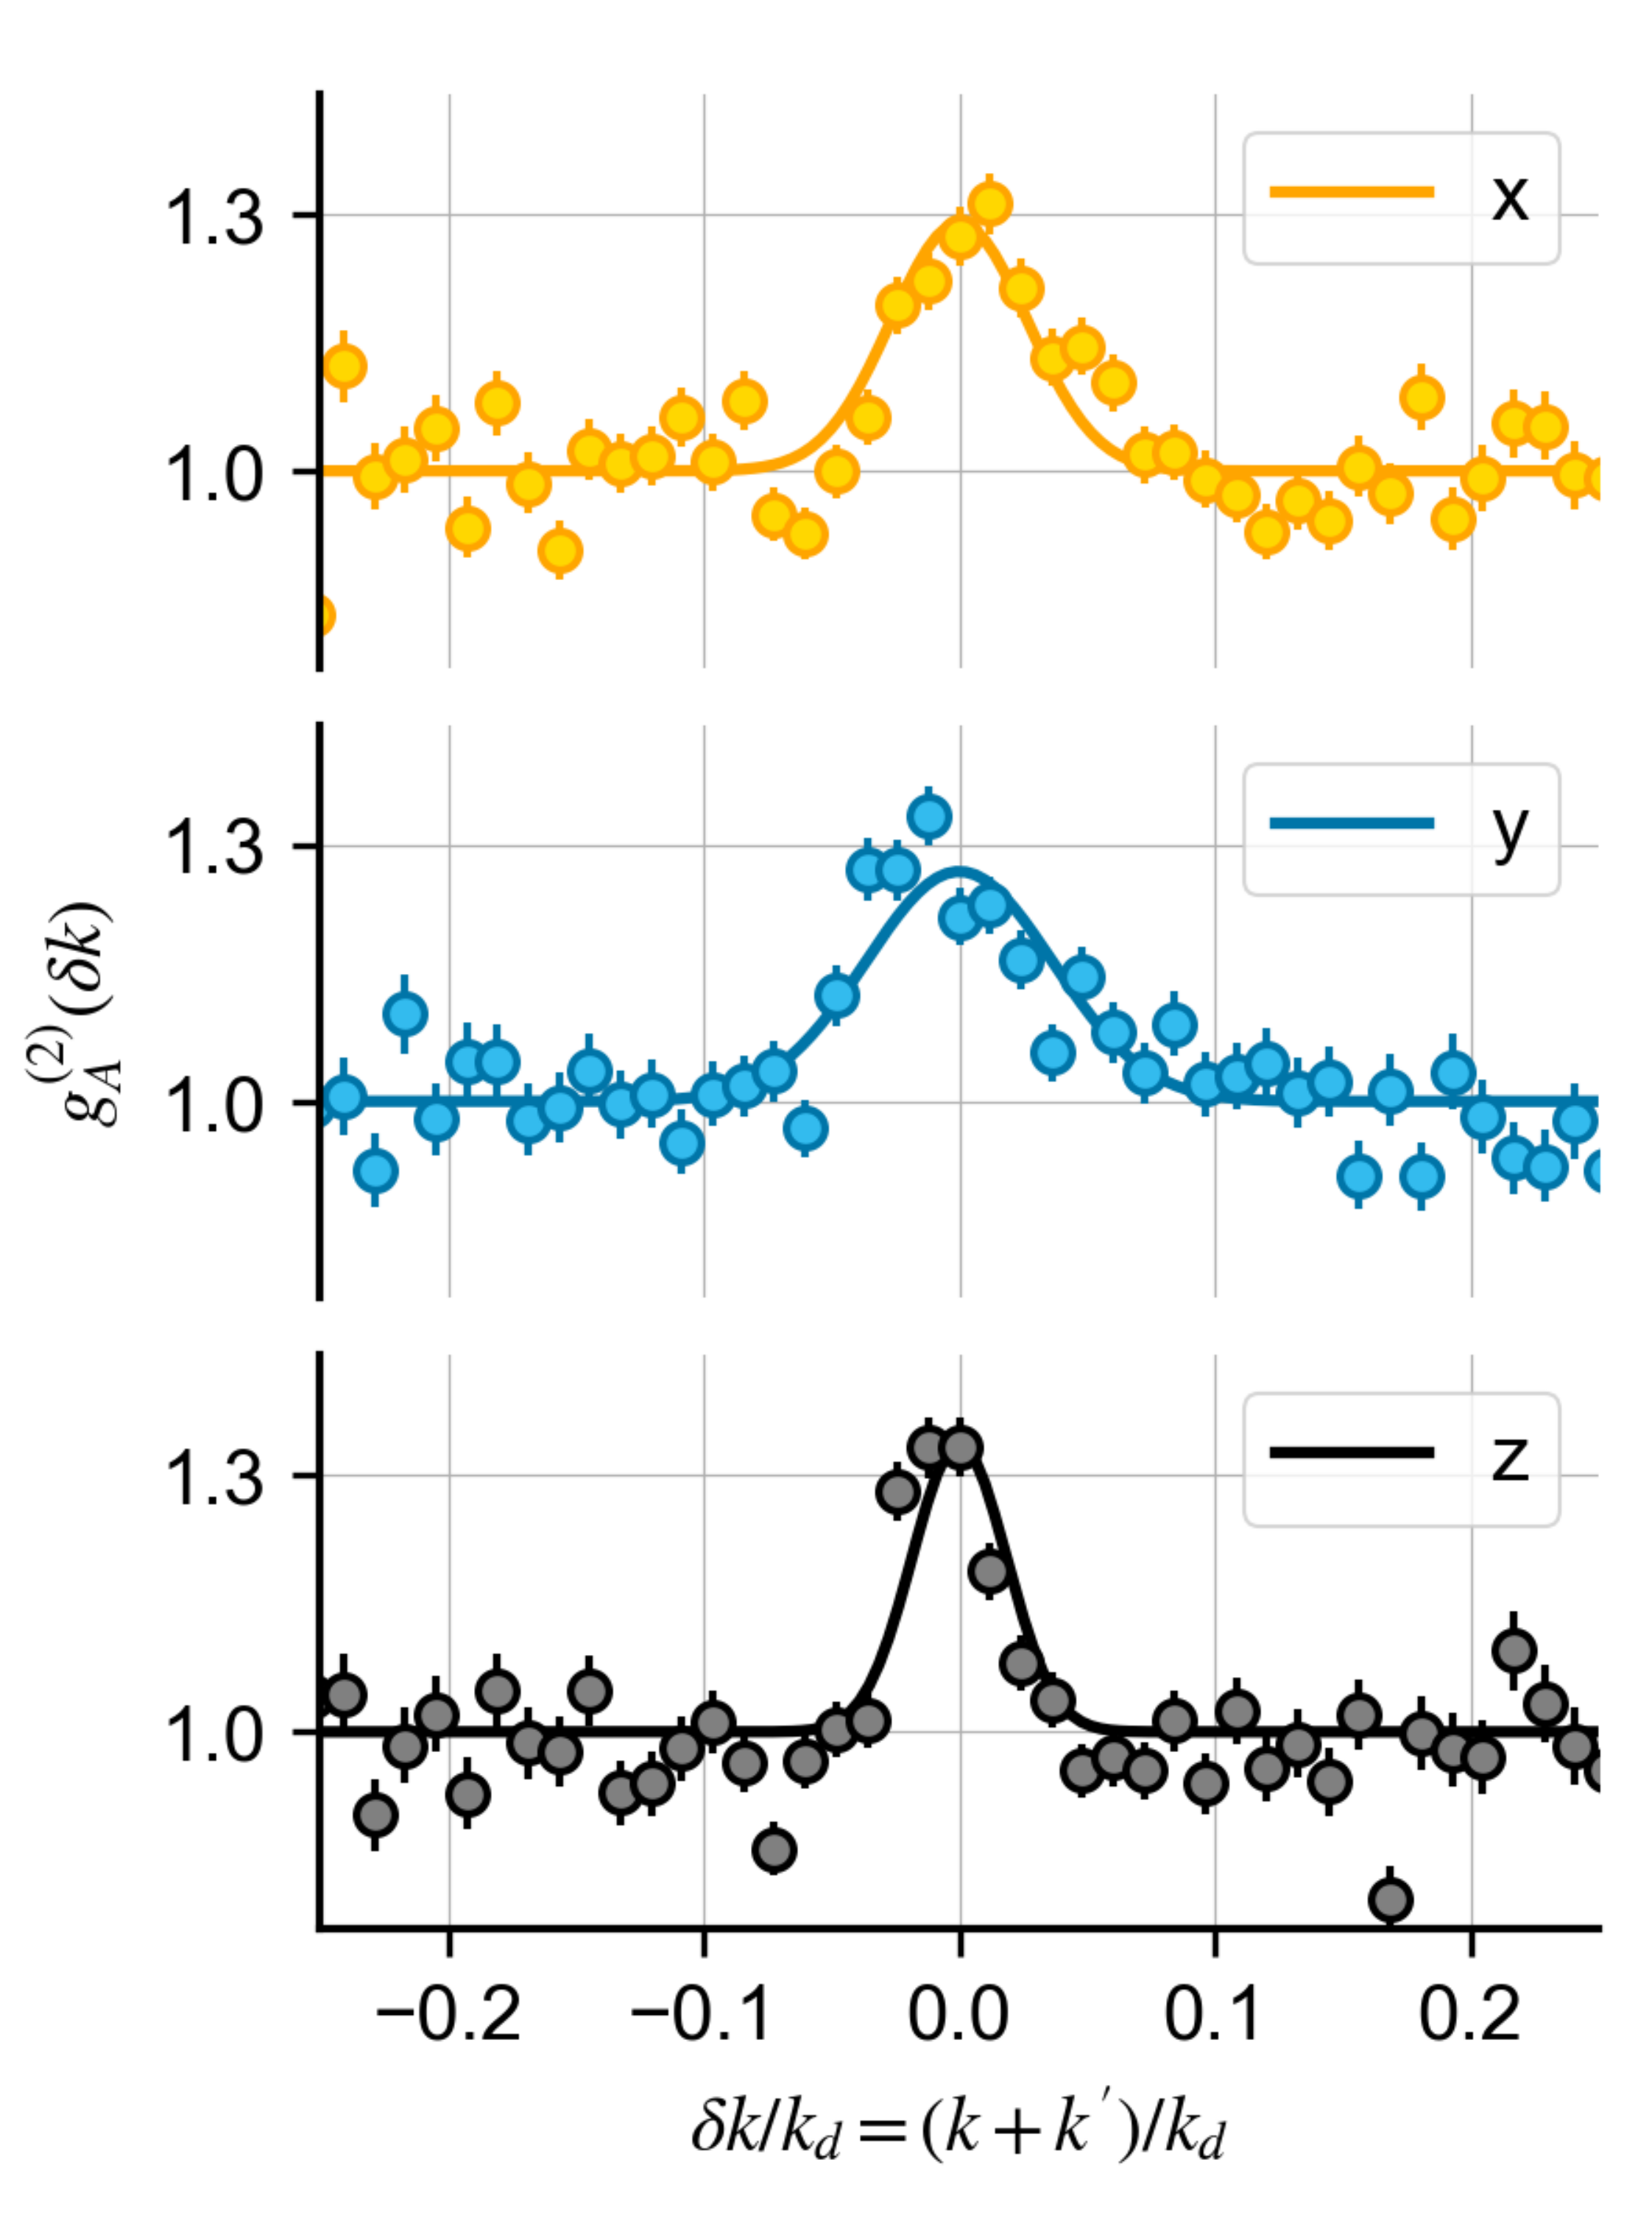
\includegraphics[width=0.65\textwidth]{Fig/Chapter4/correlations_kmk_errorbars.png}
    \caption[1D cuts through the anomalous correlation function $g_{A}^{(2)}$ along the axis of the 3D optical lattice]{1D cuts through the anomalous correlation function $g_{A}^{(2)}$ along the axis of the 3D optical lattice. The transverse integration is $\Delta k_{\perp}=3 \times 10^{-2} \ k_d$ and the longitudinal voxel size is $\Delta k_{\parallel}=1.2 \times 10^{-2} \ k_d$. The data is fitted by Gaussian functions (solid lines). The nice correlation peaks signal the presence of \kmk pairs. The error bars are obtained from the inverse square root of the number of counts in the voxels.}
    \label{fig:kmk_signal}
\end{figure}

We have plotted on Fig-\ref{fig:kmk_signal} 1D cuts through the calculated $g_{A}^{(2)}$ function on which we see clear correlation peaks standing out from the noise! This is the kind of signal we were aiming to obtain and constitutes the central result of this thesis. Before analyzing the features of this correlation signal in more details, we conduct a first series of experimental checks. First, we extend the range of $\delta \bm{k}$ on which we plot the $g_{A}^{(2)}$ function to find correlation peaks at $\delta k = \pm k_d$ as shown on Fig.-\ref{fig:periodicity}. This is something that we expected from Bloch theorem (see \ref{sec:BH_model}) as the lattice is a periodic potential.

\begin{figure}
    \centering
    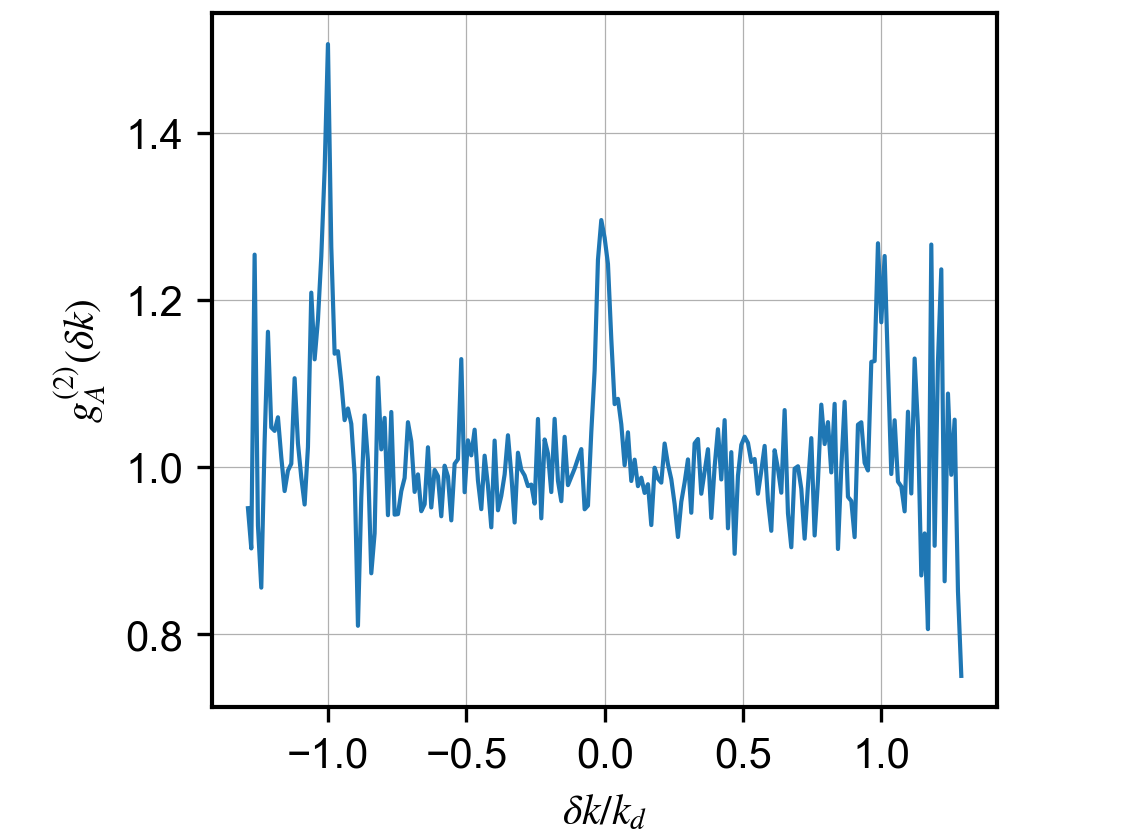
\includegraphics[width=0.7\textwidth]{Fig/Chapter4/periodicity.png}
    \caption[1D cut of the anomalous correlation function $\gtwo_A$ illustrating its periodicity]{1D cut of the anomalous correlation function $\gtwo_A$. Because of the lattice periodic potential, we observe additional correlation peaks at $\pm k_d$.}
    \label{fig:periodicity}
\end{figure}

Furthermore, we check that there are no correlations in the coherent BEC state. We do so by selecting atoms with $|k_i|<0.04 \ k_d$ with $i=x,y,z$. We show on Fig.-\ref{fig:BEC_correlations} the calculated normal and anomalous correlation functions for the mode of the BEC. As expected, both correlation functions are flat, except for a small modulation of the order of $1 \%$ that is an artifact of the normalization procedure caused by shot-to-shot fluctuations of the width of the BEC (see \cite{cayla_these}).

\begin{figure}
    \centering
    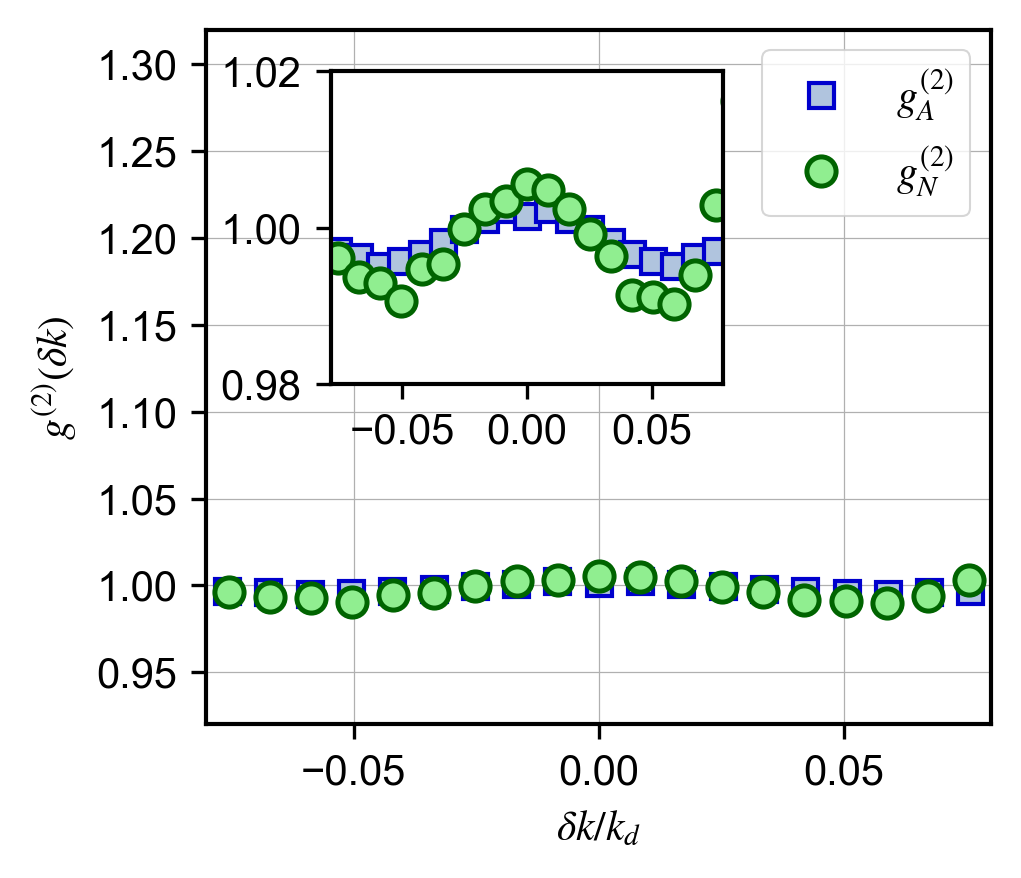
\includegraphics[width=0.65\textwidth]{Fig/Chapter4/correlations_BEC.png}
    \caption[Normal and anomalous correlation functions in the BEC]{Normal and anomalous correlation functions in the BEC. The correlation functions are flat, except for a small-amplitude modulation that is due to normalisation issues induced by shot-to-shot fluctuations of the BEC width in momentum-space.}
    \label{fig:BEC_correlations}
\end{figure}

Now that we have observed an anomalous correlation signal, we must ask whether its origin is indeed the one we expect, namely \kmk pairing in the quantum depletion as a result of the interplay between interactions and quantum fluctuations. For starters, one of the key specificity of the \kmk pairs of the quantum depletion is that they exist in an \textbf{at-equilibrium} system. This is in strong contrast with \textbf{out-of-equilibrium} configurations where non linearities efficiently drive resonant processes. In these cases, both momentum and energy are conserved and no quantum treatment is required to explain the pairing process. In fact, \kmk pairing in such systems has already been observed on various experimental platforms such as:

\begin{itemize}
    \item Parametric down conversion in quantum optics \cite{burnham1970}.
    \item Dissociation of diatomic molecules in atomic physics \cite{greiner2005}.
    \item Elastic collisions in high energy physics \cite{arnison1982} or with ultracold atoms \cite{perrin2007observation} as we have seen earlier (see Fig.-\ref{fig:kmk_kapitza}).
\end{itemize}

The main difference with the \kmk correlation signal obtained in the collision spheres is that we observe here a peak located at $\delta \bm{k} = \bm{0}$. This signals that the total momentum of the atom pair is $\bm{0}$ and as our system consists of only an at-rest BEC, the pairing process could not have resulted from an out-of-equilibrium effect. This is the novelty of our experimental observation.

While these first observations seems to point towards the fact that we are indeed seeing the \kmk pairing of the quantum depletion, we look to further characterize the correlation signal and determine whether our observations are consistent with the results of the Bogoliubov theory to prove this point. To this end, we will first study the effect of temperature that is supposed to destroy the \kmk correlation signal linked to $T=0$ quantum coherences, as explained in Chapter \ref{sec:chapter_1}.





\subsection{Effect of temperature}

\label{sec:kmk_temperature}

The temperature can be increased in a rather simple manner by holding the atoms at the final amplitude of the lattice for a longer duration, the gas being continuously heated over time (attributed to imperfections such as spontaneous emission or mechanical vibrations). We repeat the experiment with a holding time of $500 \ \rm{ms}$ corresponding to hundreds of tunneling times $225 \times h/J$. The increase in temperature can be seen by looking at the momentum density profile as shown in the panel (b) of Fig-\ref{fig:kmk_temperature}: the thermal depletion has increased, increasing the momentum density in the depletion region by a factor $\sim 4$. Note however that we did not increase the temperature too much to keep a significant condensed fraction of the order of $f_c = 29 \%$ (in the absence of BEC there is no quantum depletion). As the thermally depleted atoms show no \kmk correlations, only the denominator of equation \ref{Eq:g2_anomalous} increases as both $\rho(\bm{k})$ and $\rho(-\bm{k})$ increases each by a factor 4, thus reducing the amplitude of the anomalous correlation function by at least a factor 16, bringing it under the experimental noise as we see on Fig-\ref{fig:kmk_temperature} panel (a). Note that this reduction factor could in fact be even larger as the condensed fraction is small, meaning that the Bogoliubov approximation should not hold anymore. 

We also repeated the experiment for an intermediate temperature obtained with a holding time of $200 \ \rm{ms}$ corresponding to $90 \times h/J$ tunneling time. The condensed fraction is then $f_c=55 \%$ and we observe a peak of intermediate amplitude as shown on Fig-\ref{fig:kmk_3_temp}.

\begin{figure}
    \centering
    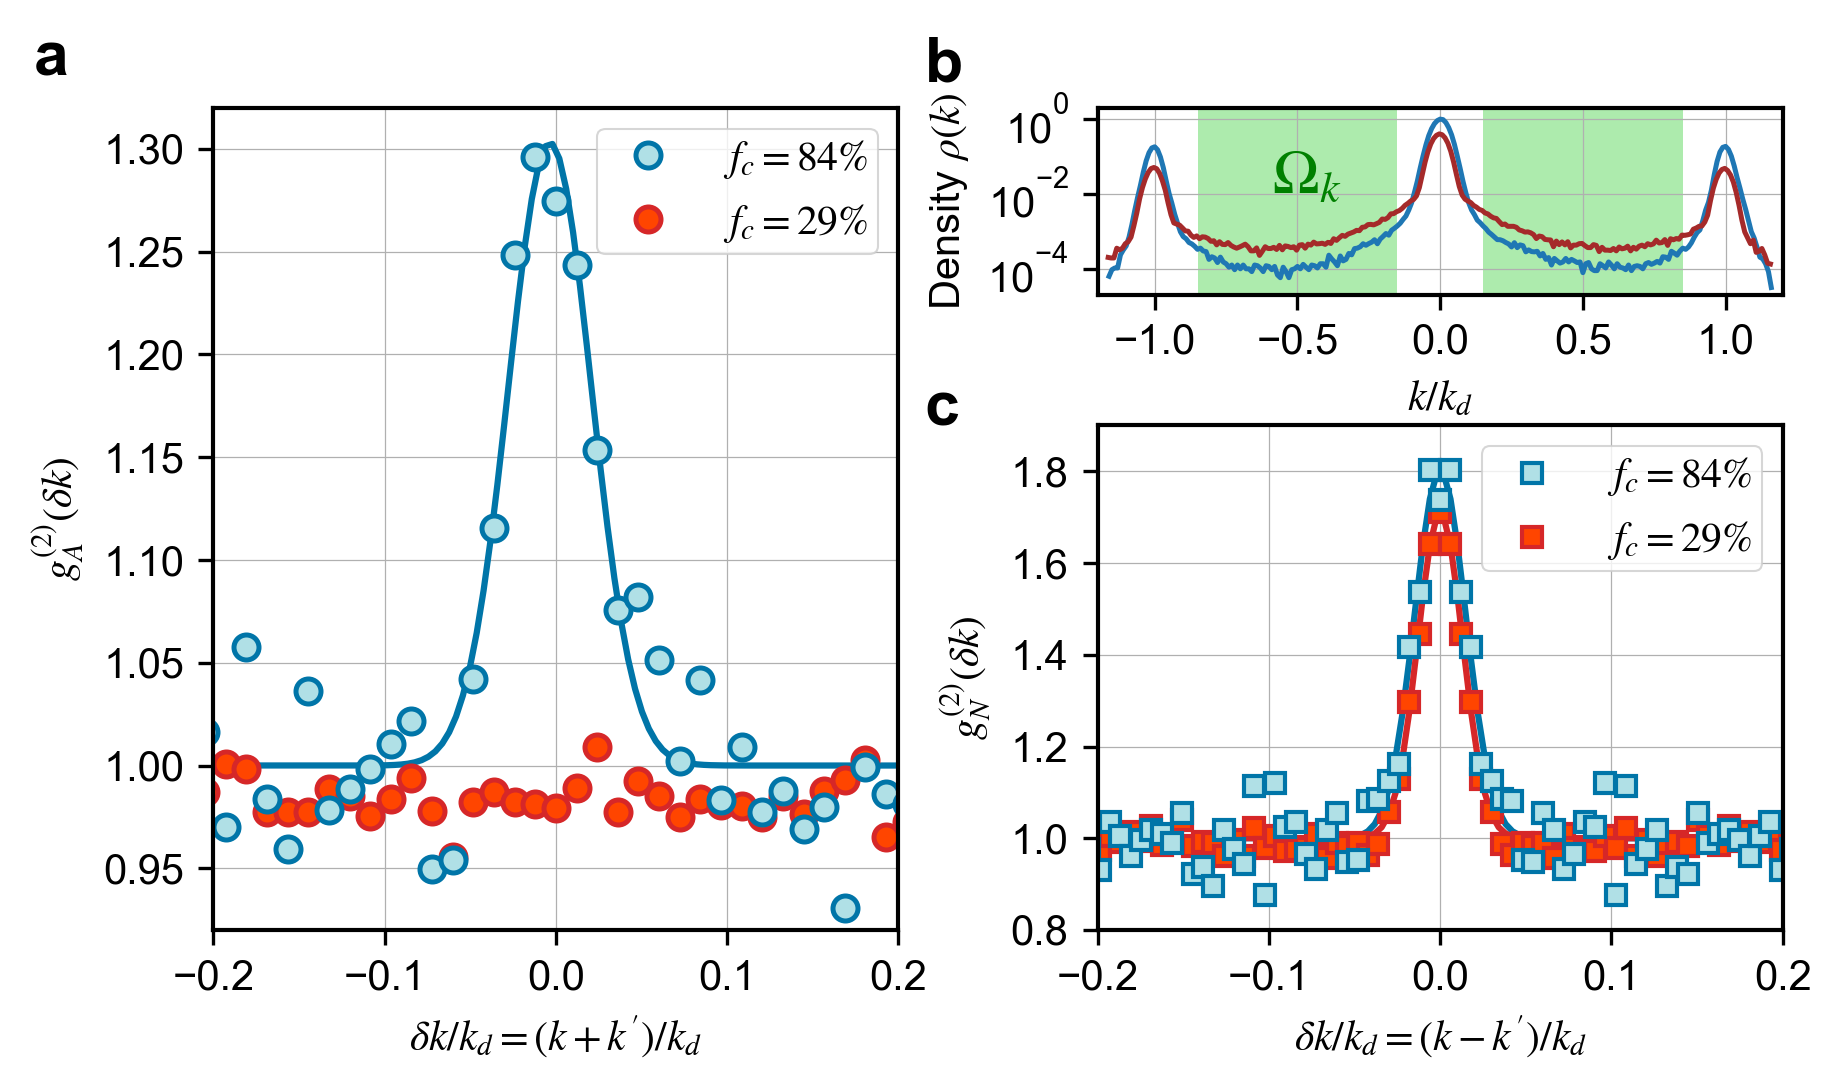
\includegraphics[width=\textwidth]{Fig/Chapter4/kmk_temperature.png}
    \caption[Atom-atom correlations in weakly-interacting BECs at two different temperatures]{Atom-atom correlations in weakly-interacting BECs at two different temperatures. The data for the low-temperature BEC ($f_{c}=84\%$), {\it resp.} for the heated BEC ($f_{c}=29\%$), are depicted in blue, {\it resp.} in red. 
    {(a)} Anomalous correlations $g_{A}^{(2)}(\delta k)$ at opposite momenta. The ${\bm k}$/$-{\bm k}$ peak disappears as the temperature increases.
    {(b)} 1D cut of the density $\rho(k)$ in semilog scale. The depletion density increases with temperature.
    {(c)} Normal correlations $g_{N}^{(2)}(\delta k)$ for the same datasets and $\Omega_k$. The peak amplitude shows no significant change as the temperature increases. Note that the transverse integration $\Delta k_{\perp}=1.5 \times 10^{-2} \, k_d$ used here reduces the amplitude of the peaks.}
    \label{fig:kmk_temperature}
\end{figure}

We thus see observe that the \kmk correlation signal is extremely sensitive to temperature, hinting to the fact that it is related to a $T=0$ ground-state effect. It is also quite illuminating to compare the \kmk correlations to the bosonic bunching \kk correlations. As explained in Chapter \ref{sec:chapter_1}, the bosonic bunching effect is the consequence of chaotic statistics, a property shared by the thermal and quantum depletion. Therefore, changing the temperature and thus the balance between thermal and quantum depletion should have no effect on bosonic bunching. This is what we observe experimentally as shown on Fig-\ref{fig:kmk_temperature} panel (c).

In conclusion, we have on the same experimental data two very different behaviours with temperature that illustrate nicely the natures of the correlation signals. On the one hand, \kk correlations unaffected by temperature, reveal the chaotic statistics of the system. On the other hand, \kmk correlations reveal the many-body ground state quantum coherences. These observations constitutes a rather convincing argument that we are indeed observing a \kmk correlation signal caused by the quantum depletion and not some other effect that we could have overlooked.

\begin{figure}
    \centering
    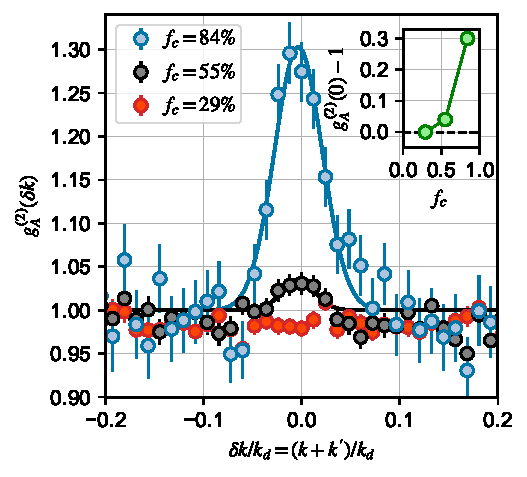
\includegraphics{Fig/Chapter4/kmk_3_temp_errorbars.pdf}
    \caption[Anomalous correlation function for data sets with different temperatures and condensed fractions]{Anomalous correlation function for data sets with different temperatures and condensed fractions. The amplitude of the $\bm{k}$/$-\bm{k}$ correlation signal is progressively lost as the temperature rises and the condensed fraction diminishes. Inset: amplitude of the correlation peak $g^{(2}_{A}({\bm 0})$ as a function of the condensed fraction $f_c$.}
    \label{fig:kmk_3_temp}
\end{figure}

In the following, we study in quantitative details these correlation signals. 


% To start on this topic, the attentive reader would have noticed than even though we expect perfect bosonic bunching $\gtwo_N (\bm{0})=2$, we rather observe $\gtwo_N (\bm{0}) \simeq 1.8$. This is due to transverse integration effects of the 3D $\gtwo$ function that need to be accounted for to extract the proper information from the amplitude of the correlation peaks.

\section{Study of the width of the correlation peaks}

\label{ref:exp_width_corr}

In a first time, we study the width of the correlation peak, a quantity that actually contains meaningful information about the many-body equilibrium state. The key aspect is the same used by Hanbury Brown and Twiss in their seminal paper to measure the size of Sirius through the measurement of the second order correlation function in far-field, namely the width of the correlation peak is inversely proportional to the spatial size of the source. 

%This argument validates our previous assumption that the correlation peak is isotropic, as the lattice trapping potential is isotropic so that the spatial size of the BEC is the same in the three directions of space.

This subject has been discussed in \ref{sec:width_correlation_theo} in light of the results of the theoretical work \cite{butera2020}. We remind that as the anomalous correlations are exclusively caused by quantum depleted atoms whose spatial extent is the one of the BEC, the width of the anomalous correlation peak $\sigma_A$ is inversely proportional to the size of the BEC $L_{\rm{BEC}}$. On the other hand, the normal correlations are caused by quantum depleted atoms but also thermally depleted atoms whose spatial size extends beyond the BEC because of the increased kinetic energy. This tells us that the width of the normal correlations peak $\sigma_N$ should be smaller than that for anomalous correlations.

\begin{figure}
    \centering
    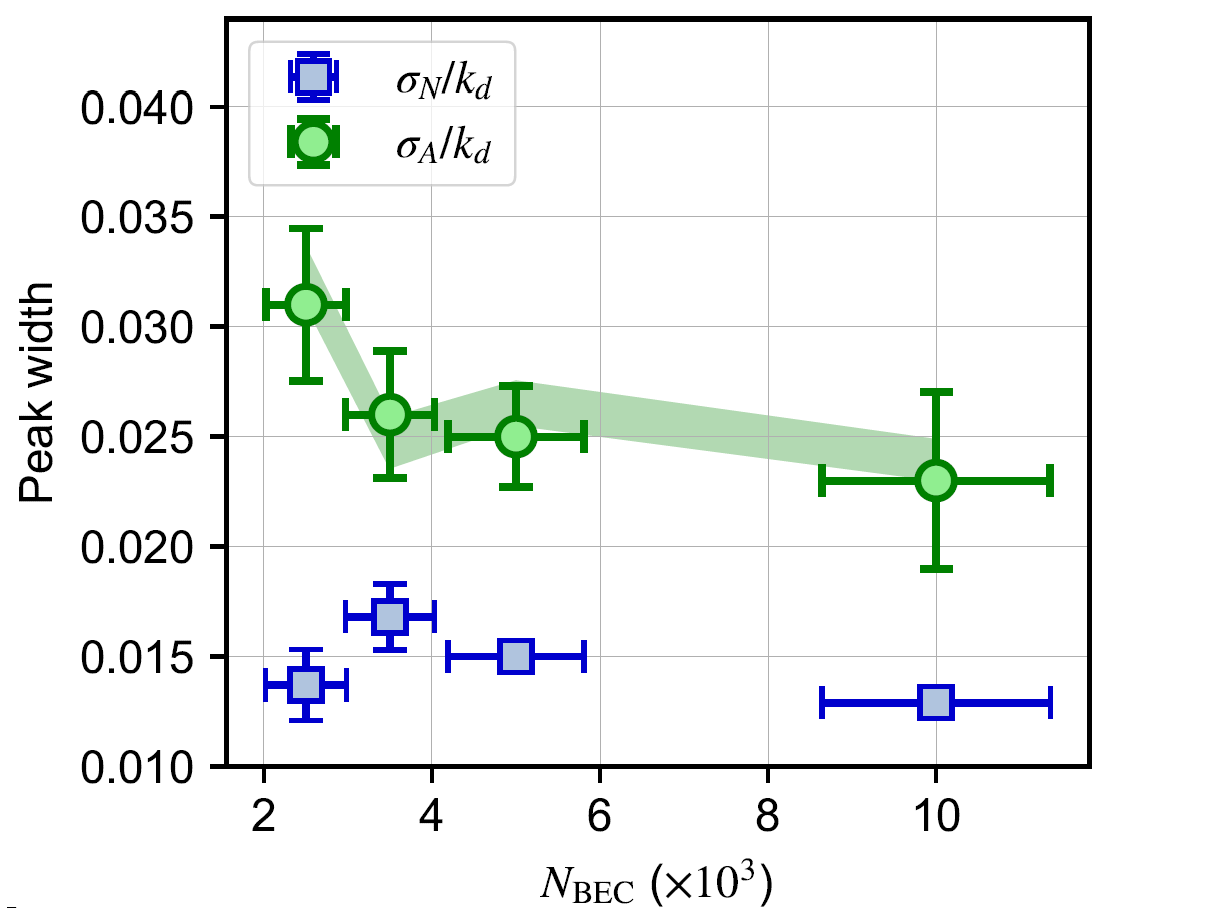
\includegraphics[width=0.65\textwidth]{Fig/Chapter4/widths.png}
    \caption[RMS widths of the anomalous and normal correlation peaks]{RMS widths of the anomalous (green) and normal (blue) correlation peaks. As expected from Bogoliubov theory, we get $\sigma_A > \sigma_N$ for each data set. The green area represents the expected with from the BEC width $\sigma_{\rm{BEC}}$ (see main text).}
    \label{fig:width}
\end{figure}

We plot on Fig.-\ref{fig:width} the experimental correlation peaks widths for different total atom numbers. The horizontal error bars correspond to the standard deviation of the total atom number, while the vertical error bars correspond to the standard deviation of the mean over the three directions of the momentum space. With this first analysis, we observe that for all atom numbers, $\sigma_A > \sigma_N$. In addition, one would expect to see both widths decrease with the total atom number as the size of the system grows with $\NBEC$. This is more or less what the experimental data suggests but the error bar are too large to make a definite statement on this point. Note that in the Thomas-Fermi regime, the size of the BEC changes slowly with the total atom number $L_{\rm{BEC}} \propto \NBEC^{1/5}$, translating in a change of $\sim 30\%$ of the width of the correlation peaks from the data with $N=2.5 \times 10^3$ to $N=10 \times 10^3$ that is hard to resolve within our error bars.

We now look at the quantitative value of $\sigma_A$ that can be numerically evaluated. The calculations have been performed by S. Butera and I. Carusotto from the BEC center in Trento, Italy, with the Bogoliubov theory for a trapped 1D system \cite{butera2020}. They evaluate $\sigma_{A,\rm{theo}} = 0.94 \sigma_{\rm{BEC}}$, with $\sigma_{\rm{BEC}}$ the RMS width in momentum space of the condensate. This relation is not modified in presence of a lattice as the size $L_{\rm{BEC}}$ does not change when the ratio $\mu/\hbar \omega$ is fixed. This is explained by the equality $m \omega^2 = m^* \omega^* ^2$ with $m^*$ the effective mass in the lattice and $\omega^*$ the corresponding effective frequency as defined in \ref{sec:rescaled_interaction}.

We can therefore measure $\sigma_{\rm{BEC}}$ to exploit this result. To do so, we need to account for deviations induced by the saturation of the detector. Indeed, the BEC is very dense resulting in a high flux of atoms saturating the detector. If we plot 1D cuts of the momentum density, the BEC momentum profile is then flattened at the top and fitting with a Gaussian function over-evaluates the momentum width of the condensate. To circumvent this issue, we adapt the parameters of the Raman transfer (see \ref{sec:raman}) to reduce drastically the flux of detected atoms and avoid saturating the detector to ensure proper fitting.

\subsubsection{Center-of-mass fluctuations}

During our first analysis, we noticed that the anomalous correlation peak was larger than that of the BEC, contrary to what we would have expected. We also noticed that the momentum width of the BEC was larger than what we obtained applying the Gutzwiller ansatz with our calibrated atom numbers. We attribute this to an imperfection in our experiment, the shot-to-shot fluctuations of the center-of-mass of the atomic distribution. When averaging over many experimental runs, these fluctuations enlarges artificially the measured width of the BEC, as well as the width of the anomalous correlation peak. These fluctuations can nevertheless be characterized by comparing the experimental momentum width of the BEC to the one predicted by the Gutzwiller variational approach.

When accounting for center-of-mass fluctuations, the measured momentum density results from the convolution with the distribution of center-of-mass displacements and has a RMS width:

\begin{equation}
    \sigma_{\rm{BEC}}=\sqrt{\sigma_{\rm{BEC},0}^2+\Delta k_{\rm{com}}^2}
\end{equation}

\noindent where $\sigma_{\rm{BEC},0}$ is the ``true'' BEC momentum width with $\sigma_{\rm{BEC},0} \propto 1/L_{\rm{BEC}}$. For instance, the Gutzwiller variational approach gives  $\sigma_{\rm{BEC},0} \simeq 1.7 \times 10^{-2} \ k_d$ for a total atom number $\NBEC = 5 \times 10^5$ and we measure $\sigma_{\rm BEC} = 2.00(4) \times 10^{-2} \ k_d$. From this we deduce $\Delta k_{\rm{com}}=1.05(2) \times 10^{-2} \ k_d$. We repeat the procedure to evaluate $\Delta k_{\rm{com}}$ for all of the data sets of Fig.-\ref{fig:width}.

For a \kmk pair of atoms, a center-of-mass displacement ${\rm{d}} \bm{k}$ induces a momentum difference $\delta \bm{k}=2 {\rm{d}} \bm{k}$. The effect of the fluctuations are thus twice larger for the width of the anomalous correlations peak than for the BEC momentum width:

\begin{equation}
    \sigma_A = \sqrt{\sigma_{A,0}^2+4\Delta k_{\rm{com}}^2}
\end{equation}

\noindent Combining this with the numerical evaluation and the measured values of $\Delta k_{\rm{com}}$, we obtain a corrected estimate of $\sigma_A$ that is represented as the green area in Fig.-\ref{fig:width}. The width of the area represent the uncertainty given by the uncertainty on the measurement of $\sigma_{\rm{BEC}}$ and the uncertainty on the determination of $L_{\rm BEC}$ caused by fluctuations of the total atom number. We find that our experimental data matches the numerical calculations of \cite{butera2020}, even if our experimental configuration is different (3D with an optical lattice contrary to 1D with a regular harmonic trap \cite{butera2020}).

We note that the fluctuations of the center-of-mass have however no effect on the normal correlation signal. Within a given shot, the center-of-mass fluctuations simply manifest as a global displacement of all the atoms of this shot by a quantity that we note $\bm{k}_{\mathrm{COM}}$. As a result, the momentum difference $\delta \bm{k} = \bm{k}_1 - \bm{k}_2$ between two atoms of this shot is not affected by the COM fluctuations, $(\bm{k}_1+\bm{k}_{\mathrm{COM}}) - (\bm{k}_2+\bm{k}_{\mathrm{COM}})=\bm{k}_1 - \bm{k}_2$. In turn, the normal correlation function $g^{(2)}_{N}(\delta \bm{k})$ remains unchanged.

We then plot again the data of \ref{fig:width} accounting for the effect of center-of-mass fluctuations. We observe that we cannot clearly state that $\sigma_A > \sigma_N$ with the experimental error bars, contrary to what we observed with our first incomplete analysis. This is most likely due to the fact the the temperature is too low to impact the width of the normal correlation function in a way that can be resolved in our experiment. 


\begin{figure}
    \centering
    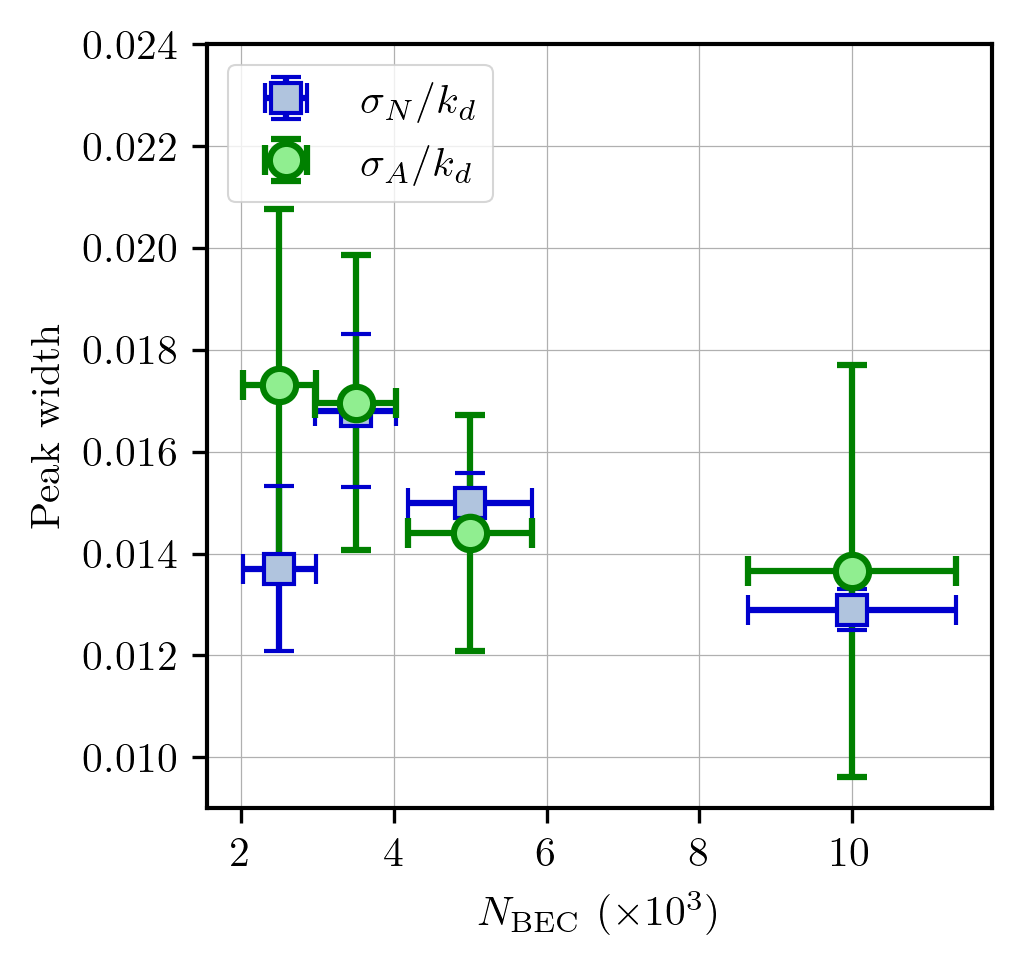
\includegraphics{Fig/Chapter4/widths_corrected.png}
    \caption[Corrected RMS widths of the anomalous and normal correlation peaks]{RMS widths of the anomalous (green) and normal (blue) correlation peaks corrected of the center-of-mass fluctuations. The widths $\sigma_A$ and $\sigma_N$ are no longer distinguishable within error bars, indicating that the temperature is too low to observe a clear separation of the anomalous and normal widths.}
    \label{fig:my_label}
\end{figure}


\section{Study of the amplitude of the correlation peaks}

We now move on to the study of the amplitude of the correlation peaks. Our objective will be to test the how the predictions of Bogoliubov theory for the homogeneous case detailled in Chapter \ref{sec:chapter_1} hold for our experimental system with an optical lattice, as well as to provide further evidence of the quantum nature of the anomalous correlation signal.


% This method is illustrated on Fig-\ref{fig:integration_kk} for the bosonic bunching measurement for two temperatures as discussed in the previous section, as well as on Fig-\ref{fig:eta_vs_int_kmk} for different anomalous correlation signals.


\subsection{Normal correlations}

The prediction of the amplitude of the normal correlation peak is straightforward: as the statistics of the system are chaotic, we should observe a perfect bunching $\gtwo_N (\bm{0})=2$.
Coming back to the normal correlations plot of Fig-\ref{fig:kmk_temperature}, we observe that the amplitude is around 1.8, \ie slightly lower than 2. This is because of the transverse integration effects described in \ref{sec:transverse_integration}. We fit the dependency of the observed amplitude with transverse integration to extract the corrected amplitude value as explained in \ref{sec:transverse_integration} and illustrated in Fig.\ref{fig:integration_kk}. We obtain $g^{(2)}_N(\bm{0})=2.05(6)$ and $g^{(2)}_N(\bm{0})=2.09(5)$ for the high and low condensed fraction data sets respectively, consistently with Bogoliubov theory showing that the statistics of the system are chaotic. Note that our team conducted a thorough study of \kk correlations in the depletion of a lattice gas in \cite{cayla2020}. 



\subsection{Anomalous correlations}

\label{sec:amp_anomalous}

We now turn to analyzing the amplitude of the anomalous correlation peaks. As we have seen with the calculations developed in section \ref{sec:amp_parametric}, we can draw an analogy between the Bogoliubov weakly-interacting Bose gas and the non-degenerate parametric amplifier in Quantum Optics. While this analogy is direct if we were to work at zero temperature and have a fully quantum depletion where all atoms are correlated, we expect in our case that the amplitude of the anomalous correlation peak is reduced because of the presence of uncorrelated thermally depleted atoms. 

We showed in \ref{sec:amp_parametric} that the amplitude of the anomalous correlation peak of the non-degenerate parametric amplifier is expected to scale linearly with the inverse of what is called the average mode occupancy, {\it i.e.} the average number of photons per mode. In atomic physics, the analog to the average mode occupancy is the momentum density, {\it i.e.} the average number of atoms in a certain mode $\bm{k}$ that we can control by changing the total number of atoms $\NBEC$. As changing $\NBEC$ should not affect the balance between the quantum and thermal depletion, we should be able to observe that the amplitude of the anomalous correlation peak scales linearly with the inverse momentum density, despite not being at $T=0$.

Acutally, as explained in \ref{sec:accessing_depletion}, we measure correlation functions averaged over many modes in the momentum volume $\Omega_k$. The parameter setting the amplitude we observe is then the average momentum density $\bar{\rho}_{\Omega_k}$ defined as:

\begin{equation}
    \bar{\rho}_{\Omega_k}=\int_{\Omega_{k}} \rho({\bm k}) {\rm d}{\bm k}
\end{equation}

We have several possibilities to change the value of $\bar{\rho}_{\Omega_k}$:

\begin{itemize}
    \item Change the experimental parameters to load a different target total atom number $\NBEC$ in the optical lattice.
    \item Change the total atom number $\NBEC$ in the post-selection (see \ref{sec:post_selec}).
    \item Change the bounds of the integration volume $\Omega_k$.
\end{itemize}

We prepare 4 data sets using a combination of these 3 possibilities. We perform the experiment with a target loaded atom number $\NBEC=[2.5,5,10] \times 10^3$, and extract an additional set with $\NBEC=3.5 \times 10^3$ from the data intended for $\NBEC = 5 \times 10^3$ by changing the post-selection criterion. We also reduce $\Omega_k$ to momenta between $k_{\rm{min}} = 0.3 \ k_d$ and $k_{\rm{max}} = 0.7 \ k_d$, {\it i.e.} to a region where the depletion is lower. We thus reduce $\bar{\rho}_{\Omega_k}$ to observe higher amplitude values in hope of observing a clear violation of the Cauchy-Schwarz inequality (see \ref{sec:cs_inequality}).

The results are plotted on Fig.-\ref{fig:amplitude_vs_rhob} alongside the normal correlations amplitude for comparison. The horizontal error bars are the same as for Fig.-\ref{fig:width} while the vertical error bars are obtained from the fit error. We observe a linear scaling of the anomalous amplitude with the inverse average momentum density. On the other side, changing $1/\rhob$ does not change the chaotic nature of the system statistics, we thus observe $\gtwo_N (\bm{0})=2$ independently of the value of $\rhob$. Once again, the amplitudes were corrected of transverse integration effects as shown on Fig.-\ref{fig:eta_vs_int_kmk}. Note that the normal correlations amplitude is not shown for the point at the lowest average density as the amplitude does not increase at lower densities, resulting in a decrease of the signal-to-noise ratio.

\begin{figure}
    \centering
    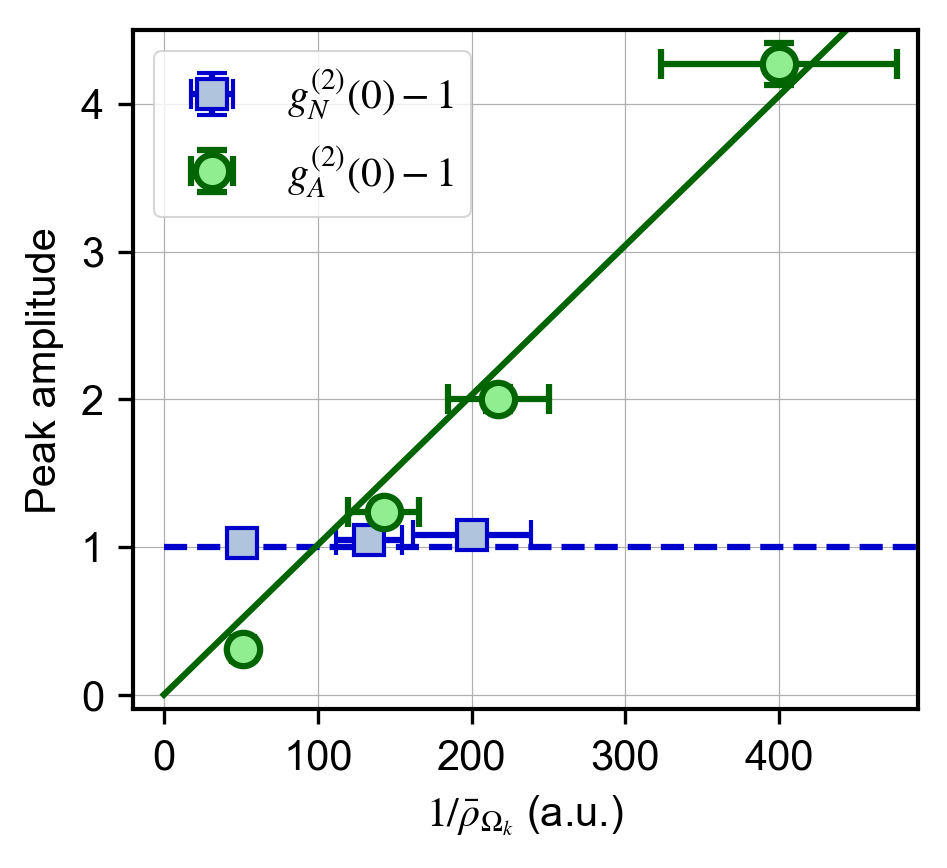
\includegraphics[width=0.65\textwidth]{Fig/Chapter4/amplitude_kmk.png}
    \caption[Amplitude of the correlation peaks versus the inverse average density $\rhob$]{Amplitude of the correlation peaks versus the inverse average density $\rhob$. We observe a linear scaling for anomalous correlations, while normal correlations stay constant and compatible with $\gtwo_N (\bm{0})=2$.}
    \label{fig:amplitude_vs_rhob}
\end{figure}

If we were at $T=0$, we remind from \ref{sec:amp_parametric} that the absolute value of the amplitude of the anomalous correlation peak should be $\gtwo_A (\bm{0}) = 2 + 1/\rhob$. Because of the temperature, we rather expect that the limit of $\gtwo_A (\bm{0})$ when $\rhob$ goes to infinity is a number between 1 and 2 whose value is determined by the balance between the quantum and thermal depletion. In the experiment, we found that a linear fit of $\gtwo_A (\bm{0})-1$ versus $1/\rhob$ with a zero intercept well matches the data, suggesting that the fraction of quantum depletion is actually very small. In fact, this quantity can be determined more precisely as we will now see.


\subsubsection{Discussion on the detected number of atom pairs}

The absolute value of the amplitude can be used to extract the number of detected \kmk pairs, following the procedure previously described in \ref{sec:benchmark_algo}. For the data set $\NBEC=5 \times 10^3$, $f_c=84 \%$, we find that we detect on average $0.5$ pairs per shot, for roughly $N_{\Omega_k}=100$ atoms detected in $\Omega_k$. This number can be used to calculate the fraction of quantum depleted atoms in the overall depletion condensate that we will write $\alpha_Q$. We first assume that all atoms in the quantum depletion form a \kmk pair and that atoms forming a \kmk pair necessarily belong to the quantum depletion. We then have:

\begin{equation}
    2N_{\rm{pairs}}= N_{\Omega_k} \alpha_{\rm{MCP}} \alpha_Q
    \label{eq:Npairs}
\end{equation}

\noindent This equation can be understood as follows. We initially have a given number of depleted atoms in $\Omega_k$ that we detect only a fraction of because of the MCP detection efficiency. This number is $N_{\Omega_k}$. In all these atoms, only the fraction of quantum depleted ones $\alpha_Q$ will be \kmk paired. In addition, we miss some pairs when detecting only one atom of the pair because of the detection efficiency, hence the addition of $\alpha_{\rm{MCP}}$ in the formula.

We use equation \ref{eq:Npairs} to evaluate $\alpha_Q$ and find $\alpha_Q \simeq 1.6 \%$. Using a $T=0$ Gutzwiller approach (see \ref{sec:gutzwiller}), we estimate the quantum depletion to be $5\%$ and infer that the thermal depletion must then be $\simeq 10\%$ as the overall condensed fraction is $f_c=84 \%$. This would mean that we should rather have $\alpha_Q \simeq 33 \%$, so more than an order of magnitude larger than our experimental measurement. We perform the same measurements for data sets with different total atom numbers with the results shown in Table-\ref{tab:nb_pairs}, and observe that the value of $\alpha_Q$ does not significantly change. While this is consistent with the fact that we are able to observe a linear scaling of $\gtwo_A (\bm{0})$ with $1/\rhob$ and that $\gtwo_A (\bm{0})-1$ tends to almost zero when $1/\rhob$ goes to infinity, there is significant discrepancy with the estimation of the Gutzwiller approach. Finding a clear explanation for this discrepancy remains an open question and would require an extensive theoretical work far beyond the scope of this thesis. We can however suggests a few possible explanations:

\begin{itemize}
    \item While we estimate the total quantum depletion, we cannot count all the pairs as some of them are located in the region of the BEC removed from the analysis. At the moment, we do not have the theoretical tools necessary to determine how many pairs are removed that way.
    \item Some of the pairs that we detect are located close to the edge of the first Brillouin where the relation dispersion becomes flat. It is then not so clear whether Bogoliubov's theory predictions for an homogeneous gas should hold, as the Bogoliubov dispersion relation is an increasing function of the momentum.
    % \item The balance between thermal and quantum depletion depends from the momentum $k$. It is then not so clear of what this number should be averaged over $\Omega_k$. In addition, a significant amount of \kmk pairs can be located in the low $k$ region that we remove from the analysis, thus reducing the number of detected pairs.
    % \item Dispersion relation of the lattice \NOTE{COMPLETER}
    % \item Is is also not so clear how the pairs are projected into the different Brillouin zones when performing the time-of-flight measurement. This could also makes us miss some pairs (\NOTE{BOF}).
\end{itemize}

\begin{table}[]
    \centering
    {\rowcolors{2}{white}{MainColor!12}
    \begin{tabular}{ c|c|c }
        {\color{MainColor} $\bm{N_{\rm{BEC}}}$} & {\color{MainColor} $\bm{N_{\rm{pairs}}/N_{\rm{runs}}}$} & {\color{MainColor} $\bm{\alpha_Q$}}  \\
        $2.5 \times 10^3$ & $0.15$ & $1.5 \%$ \\ 
        $5 \times 10^3$ & $0.5$ & $1.6 \%$ \\ 
        $10 \times 10^3$ & $0.9$ & $1.2 \%$ \\ 
    \end{tabular}}
    \caption{Average number of detected \kmk pairs per experimental run and fraction of quantum depleted atoms in the depletion for different total atom numbers.}
    \label{tab:nb_pairs}
\end{table}



In conclusion, the observed linear scaling is consistent with what is predicted by Bogoliubov theory and gives us another argument showing that the observed anomalous correlation signal is linked to the quantum depletion. The absolute value of the amplitude cannot however be understood in the framework of the Bogoliubov theory \cite{butera2020} that does not account for all the specificities of our experiment, such as the presence of the lattice. In fact, evaluating this number is currently beyond what is possible to calculate, making our experiment an example of quantum simulation.


\section{Towards measuring entanglement}

As we underlined in the first chapter of this thesis, it would be of great interest to characterize how entanglement emerges in at-equilibrium many-body systems such as the one we are working with here. Although we do not have all the experimental tools to claim that we are indeed seeing entanglement in our experiment yet, we nevertheless observe clear signatures of quantum phenomena that hints towards it as we will discuss now.



\subsection{Relative number squeezing}

As detailled in paragraph \ref{sec:correlated_pop} of Chapter \ref{sec:chapter_1}, if we were in the perfect situation $T=0$ were the depletion is fully quantum, the populations in modes $\bm{k}$ and $-\bm{k}$ would be totally correlated so that the quantity $N(\bm{k})-N(-\bm{k})$ is non-fluctuating and always equal to 0. This is obviously not the case in our finite temperature experiment where a significant fraction of the depletion is thermal and thus uncorrelated. However, we expect the \kmk correlations to reduce the fluctuations of $N(\bm{k})-N(-\bm{k})$. This is what we call \textbf{relative number squeezing}, similar to --but not to be confused with-- regular squeezing \cite{walls1983squeezed} that denotes the reduction of the fluctuations of an operator ({\it e.g} momentum) under the Heisenberg limit at the expense of increased fluctuations for the conjugate operator ({\it e.g} position).

% A slightly higher level proof of quantum behavior than the violation of the Cauchy-Schwarz inequality is observing \textbf{squeezing}. Before going into our experimental details and observations, let us briefly remind what is squeezing is.

% In quantum mechanics, the maximum precision with which one can hope to measure two conjugate quantities such as position and momentum is bound by the very famous Heisenberg inequality:

% \begin{equation}
%     \Delta x \Delta p \geq \frac{\hbar}{2}
% \end{equation}

% In most cases, notably the quantum harmonic oscillator ground state $\ket{0}$ and coherent states $\ket{\alpha}$, the minimum uncertainties values saturating the Hesienberg inequality are the same for the two conjugate quantities $\Delta x_{g} = \Delta p_g$. The specificity of squeezed states is that the uncertainty one of the quantities has been reduced below the lower limit of the ground state, at the detriment of the uncertainty of the conjugate quantity. If we were to represent the uncertainty in quadrature space, we would get a perfect circle for a coherent state and a "squeezed" circle, {\it i.e.} an ellipse, for a squeezed state, hence the name. \NOTE{BIBLIO/EXEMPLES}, \NOTE{VOIR AVEC CHAPITRE 1 OU METTRE CA}

% A well-known example of how to obtain squeezing is the non degenerate parametric amplifier in non linear quantum optics. \NOTE{A faire quand le chapitre 1 est fait}

 The idea is then to measure the statistics of the difference of atom numbers in modes $\bm{k}$ and $-\bm{k}$ that we will refer to as $N(\bm{k})$ and $N(-\bm{k})$. For one of the modes, the fluctuations of the number of atoms are set by the \textbf{shot noise} and follow a Poisson law. The particularity of the Poisson law for a random variable is that the variance of the variable is equal to its mean, giving for instance for mode $\bm{k}$:

\begin{equation}
    \sigma_{N(\bm{k})}^2 =\mean{N(\bm{k})^2}-\mean{N(\bm{k})}^2 = \mean{N(\bm{k})}
\end{equation}

What can we tell of the statistics of the number difference in two modes $\bm{k}$ and $\bm{k}'$, $N(\bm{k}) - N(\bm{k}')$? If the populations in the two modes are totally uncorrelated, the difference of two independent Poissonian random variables is Poissonian as well and we then get:

\begin{equation}
    \sigma_{N(\bm{k})-N(\bm{k}')}^2 = \mean{N(\bm{k})-N(\bm{k}')}
\end{equation}

If we now chose $\bm{k}'=-\bm{k}$, we expect the \kmk correlations present in the depletion to reduce the fluctuations of the number difference, yielding what is called a \textbf{sub-Poissonian} law. Just like the \kmk correlation signal is lost with temperature, we expect that the reduction of the number difference fluctuations becomes smaller and smaller as temperature increases, increasing the fraction of thermally, uncorrelated, depleted atoms. 

Our goal is then to measure $\sigma_{N(\bm{k})-N(-\bm{k})}$ and see whether it is smaller than the expected value for a Poisson law. To this end, we define a convenient quantity that we call the squeezing parameter $\xi$: 

\begin{equation}
    \xi_{\bm{k},\bm{k'}}^2=\frac{\langle (N_{\bm{k}} - N_{\bm{k'}})^2 \rangle - \langle N_{\bm{k}} - N_{\bm{k'}} \rangle^2}{\langle N_{\bm{k}} \rangle + \langle N_{\bm{k'}} \rangle}
\end{equation}

This squeezing parameter to the square is simply the standard deviation of the number difference normalized by the expected standard deviation for uncorrelated variables. Therefore, we expect $\xi^2_{\bm{k},\bm{k}'}=1$ if there are no correlations between modes $\bm{k}$ and $\bm{k'}$, and $\xi^2_{\bm{k},\bm{k}'} < 1$ if the modes populations are correlated.

To evaluate $\xi^2$, we record for each experimental shots the number of detected atoms in cubic boxes paving the entire integration volume $\Omega_k$. Intuitively, we could set the size of the boxes to match that of a mode. If we define the volume of a mode as the volume of a sphere whose radius is the two-particle correlation length $l_c$ obtained from the normal correlation function width with $l_c = \sqrt{2} \sigma_N$ \cite{carcy2019momentum}, we obtain that there are $N_{\rm{mode}} = 1.5 \times 10^4$ modes in $\Omega_k$, \ie on average $\sim 0.01 \ \text{atoms/mode/run}$ (for $\NBEC=5 \times 10^3$) which is way to small to have proper statistics to evaluate $\xi^2$. We then chose a size of $(0.3 \ k_d)^3$. The average numbers of detected atoms per shot are $\sim 100$, $\sim 240$ and $\sim 360$ for the data sets with $f_c=84\%$, $f_c=55\%$ and $f_c=29\%$ respectively, meaning that the average number of atom per box are $0.8$, $1.92$ and $2.88$ respectively. Having access to the atom number for each of the $\sim 2000$ runs at various values of $\bm{k}$, we compute the squeezing parameter between different pairs of boxes as illustrated on Fig.-\ref{fig:squeezing}, either correlated or uncorrelated for reference. The measured values of $\xi^2$ are averaged over all possible pairs of boxes for a given configuration. The uncertainty on $\xi^2$ is evaluated statistically on all the $\xi^2$ values obtained on the 62 different pairs of boxes and defined as the standard error.

\begin{figure}
    \centering
    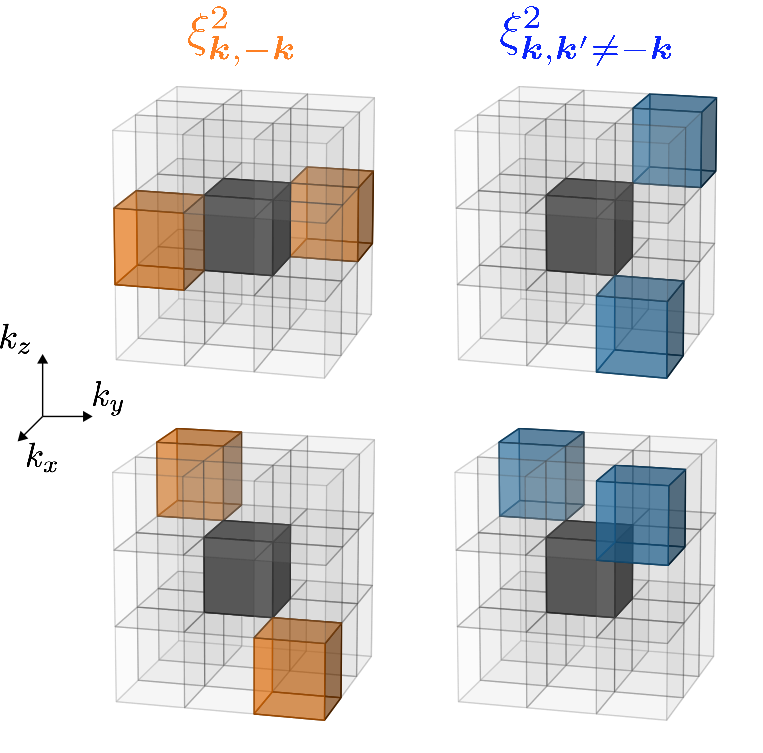
\includegraphics[width=0.7\textwidth]{Fig/Chapter4/squeezing.png}
    \caption[Relative number squeezing measurement]{Relative number squeezing measurement. The number of detected atoms in cubic boxes are recorded for each experimental run. We compute the squeezing parameter $\xi$ between correlated (orange) boxes as illustrated on the right, or uncorrelated (blue) boxes on the left. The central black box corresponds to the BEC, removed from the analysis.}
    \label{fig:squeezing}
\end{figure}

The results are summarized in Table \ref{tab:squeezing}. For the low-temperature, high condensed fraction data, we are indeed able to observe a small relative number squeezing within the errorbars. Note that this number squeezing is small compared to that found in discrete (spin) variables experiments \cite{bucker2011,esteve2008squeezing, pezze2018} as it is inherently limited by the uncorrelated thermally depleted atoms and the detection efficiency. For uncorrelated modes, the squeezing parameter is very slightly above 1, highlighting that the correlations indeed reduce the fluctuations of the number difference. For higher temperatures (lower condensed fraction), no relative number squeezing is observed as the correlations are drowned out. In addition, we see that the squeezing parameter increases as we increase the temperature. This is due to global atom number fluctuations of the order of $15\%$ in our experiment. At low temperature, there are few detected atoms er box and the shot noise is thus large and dominating the total atom number fluctuations. On the opposite, at higher temperatures, the number of depleted atoms increases, reducing the shot noise. The contribution of total atom number fluctuations is then not negligible anymore and increase the fluctuations of the number difference, higher than what is expected for a Poisson law, explaining why we observe $\xi^2 > 1$.

\begin{table}[ht!]
    \centering
    {\rowcolors{2}{white}{MainColor!12}
    \begin{tabular}{ c|c|c }
        {\color{MainColor} $f_c$} & {\color{MainColor}$\xi^2_{\bm{k},-\bm{k}}$ } & {\color{MainColor}$\xi^2_{\bm{k},\bm{k}'}$} \\
        0.84 & 0.992(3) & 1.004(3) \\
        0.55 & 1.017(4) & 1.017(3) \\
        0.29 & 1.040(5) & 1.045(5) \\

    \end{tabular}}
    \caption{Experimental values of the squeezing parameter for correlated and uncorrelated modes and different condensed fractions.}
    \label{tab:squeezing}
\end{table}


% \begin{table}[]
%     \arrayrulecolor{black}
%     \centering
%     \begin{tabular}{|c|c|c|}
%         \hline
%         $f_c$ & $\xi^2_{\bm{k},-\bm{k}}$ & $\xi^2_{\bm{k},\bm{k}}$ \\
%         \hline
%         0.84 & 0.992(3) & 1.004(3) \\
%         \hline
%         0.55 & 1.017(4) & 1.017(3) \\
%         \hline
%         0.29 & 1.040(5) & 1.045(5) \\
%         \hline
%     \end{tabular}
%     \caption{Experimental values of the squeezing parameter for correlated and uncorrelated modes and different condensed fractions.}
%     \label{tab:squeezing}
% \end{table}

\subsection{Experimental violation of the Cauchy-Schwarz inequality}

We have previously shown in \ref{sec:cs_inequality} how the Cauchy-Schwarz inequality writes with creation and annihilation operators and translated it in terms of correlation functions. We remind that we obtained:

\begin{equation}
    \gtwo_A (\bm{k},-\bm{k}) \leq \gtwo_N (\bm{k},\bm{k})
\end{equation}

We thus have a clear violation of the Cauchy-Schwarz inequality with our experimental data on 3 different data points, with a maximum violation of $5.27(8) > 2$ (Fig.-\ref{fig:amplitude_vs_rhob}). This adds up to the list of quantum signatures in the anomalous correlation signal.

As discussed in \ref{sec:cs_inequality}, violating the Cauchy-Schwarz inequality equals fulfilling the Busch-Parentani criterion to prove entanglement, provided that certain conditions are fulfilled. The first one is that the statistics of the system must be thermal chaotic. This is something that we have experimentally verified by measuring $\gtwo_N (\bm{0}) = 2$. The second condition is to have $\langle a^{\dagger}({\bm k}) a({-\bm k}) \rangle=0$. While this is true in Bogoliubov theory and would be reasonable to assume in our experiment, this is not something that we have experimentally measured and that therefore forbids us to claim that we observe entanglement in momentum space. While we do not have at the moment the experimental tools necessary to measure $\langle a^{\dagger}({\bm k}) a({-\bm k}) \rangle$, proving the presence of entanglement in momentum space in many-body ground states would be a significant result that motivates the improvement of our experimental setup in the near future. \NOTE{how}

% The very famous Cauchy-Schwarz inequality has seen countless applications in mathematics and physics. What will most interest us here is its formulation in the framework in probability theory. In classical physics, with two fluctuating quantities $I_1$ and $I_2$, the Cauchy-Schwarz inequality writes:

% \begin{equation}
%     \mean{I_1 I_2} \leq \sqrt{\mean{I_1^2} \mean{I_2^2}}
% \end{equation}

% This inequality can be rewritten with creation/annihilation operators to work with two-body correlation functions. For simplicity sake, let's consider only two modes 1 and 2. We introduce the notation $G^{(2)}_{i,j} = \mean{\hat{a}(i)^{\dagger} \hat{a}(j)^{\dagger} \hat{a}(i) \hat{a}(j)}$. The Cauchy-Schwarz inequality becomes \cite{kheruntsyan2012violation,walls2008}:

% \begin{equation}
%     G^{(2)}_{1,2} \leq \sqrt{G^{(2)}_{1,1} G^{(2)}_{2,2} }
% \end{equation}

% If we now chose mode $1 \rightarrow \bm{k}$, mode $2 \rightarrow -\bm{k}$ and consider a symmetrical case with $\mean{\hat{a}^{\dagger}(\bm{k}) \hat{a}(\bm{k})}=\mean{\hat{a}^{\dagger}(-\bm{k}) \hat{a}(-\bm{k})}$ (consistent at $T=0$ where the depletion is fully quantum and exclusively populated in pairs), we obtain $G^{(2)}_{\bm{k},\bm{k}}=G^{(2)}_{-\bm{k},-\bm{k}}$ and finally:

% \begin{equation}
%     \gtwo_A (\bm{k},\bm{-k}) \leq \gtwo_N (\bm{k},\bm{k})
% \end{equation}

% Therefore, the Cauchy-Schwarz inequality states that the cross-correlation amplitude between opposite momenta cannot exceed the amplitude of the auto-correlation with a classical model. As shown on Fig-.\ref{fig:amplitude_vs_rhob}, the experimental amplitude of the anomalous correlations goes significantly higher than for normal correlations, thus clearly violating the Cauchy-Schwarz inequality for classical quantities: we are thus observing quantum correlations. As developed in \cite{kheruntsyan2012violation}, violating the Cauchy-Schwarz inequality is one of the easiest way to prove the presence of non-classical correlations and represents a first, necessary step towards obtaining more significant results such as proving the presence of entanglement.

\section{Preliminary study: dependency of the correlation signals with k}

As we have seen throughout this chapter, the balance between the quantum and thermal depletion and thus the temperature plays an important role in both the amplitude of the anomalous correlation function (see \ref{sec:kmk_temperature}) as well as the width of the normal correlation function (see \ref{sec:width_correlation_theo}). Interestingly, the ratio of the quantum and thermal depletion changes with the momentum value $k$ as they have different momentum scales set by the strength of the interactions and the temperature respectively. Whereas we have until now kept the integration volume $\Omega_k$ as large as possible, it would be then be interesting to reduce it and move it around momentum space to see whether we can observe variations of the characteristics of the correlation signals depending on the momentum value around which $\Omega_k$ is centered. Note that the study presented in this section is preliminary and still an on-going work.

\subsection{Evolution of the amplitude of the anomalous correlations with k}

As far as the amplitudes of the correlation signals are concerned, there is not much too learn studying the dependency of the amplitude of the normal correlation signal with $k$ as it only reveals the chaotic statistics of the system that are unaffected by temperature and are thus independent of $k$. We will then focus solely on the amplitude of the anomalous correlation function. 

We repeat the analysis procedure described before for various integration volumes $\Omega_k$ that we set by changing its boundaries $k_{\rm{min}}$ and $k_{\rm{max}}$ (see \ref{sec:accessing_depletion}). In practice, we chose the couples $[k_{\rm{min}},k_{\rm{max}}]=[0.15,0.3],[0.2,0.35],...,[0.35,0.5] \ k_d$, scanning the first Brillouin zone. As $\Omega_k$ is smaller than for previous analysis showed in this chapter, the signal to noise ratio is not sufficient to extract a value of the amplitude for a large panel of transverse integration values to extract the amplitude corrected from transverse integration as described in \ref{sec:transverse_integration}. We will then rather plot the raw amplitude $\eta_A$ for a fixed transverse integration $\Delta k_{\perp}=3 \times 10^{-2} \ k_d$. In addition, when changing $\Omega_k$, we also change the value of $\rhob$ that affects the amplitude of the anomalous correlation peak. We therefore ``normalize'' this effect by plotting the quantity $\eta_A \times \rhob$ that should only reveal the effect of the variations of the balance between the quantum and the thermal depletion.

We plot on Fig.-\ref{fig:eta_A_vs_k} $\eta_A \times \rhob$ as a function of $k_{\rm{center}}=(k_{\rm{min}}+k_{\rm{max}})/2$ for the data sets with $\NBEC= 5 \times 10^3$ and holding times $5 \ \rm{ms}$ and $200 \ \rm{ms}$. We observe that for the coldest data set, $\eta_A \times \rhob$ increases with $k$, indicating that the ratio of the quantum depletion to the thermal depletion increases with $k$ in the momentum range that we probe. When the temperature increases (orange points of Fig.-\ref{fig:eta_A_vs_k}), the thermal depletion increases and populates higher momentum modes, meaning that the ratio of the quantum depletion to thermal depletion should not increase as fast or even possibly decrease with $k$ if the temperature is high enough. This is what we observe on the experimental data for which $\eta_A \times \rhob$ increases much slower for the heated data. We note that as the overall density of the depletion is higher at low $k$ reducing the amplitude of the anomalous correlation function, we were not able to observe the correlation signal for $[k_{\rm{min}},k_{\rm{max}}]=[0.15,0.3],[0.2,0.35]$ with the $200 \ \rm{ms}$ holding data.

\begin{figure}
    \centering
    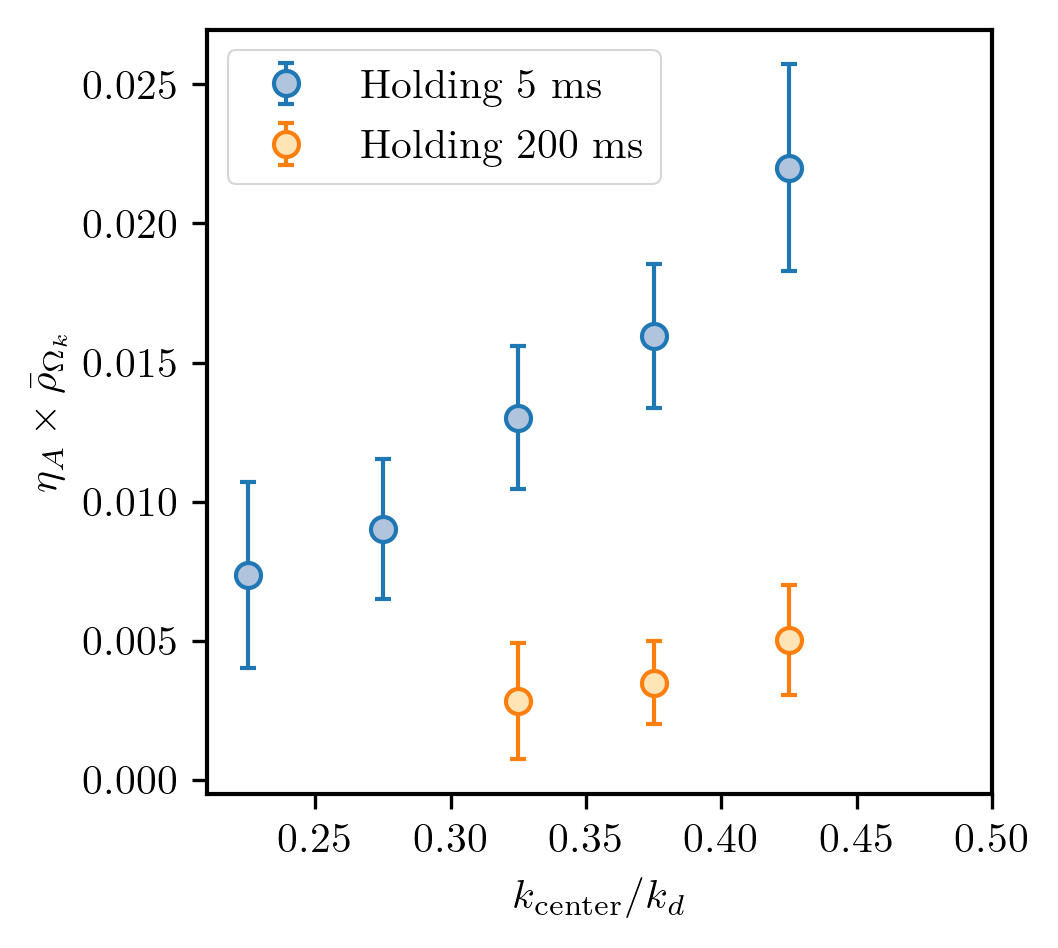
\includegraphics[width=0.7\textwidth]{Fig/Chapter4/eta_A_vs_k.png}
    \caption[Evolution of the anomalous correlations amplitudes with $k$]{Raw amplitude $\eta_A$ mutiplied by the average density $\rhob$ as a function of $k_{\rm{center}}$ for two data sets as different temperatures.}
    \label{fig:eta_A_vs_k}
\end{figure}

While this kind of data could in principle be used to find the temperature of the experiment, we must for the moment only restrict ourselves to the qualitative description we have just given for lack of a precise theory of the correlations in an optical lattice.

\subsection{Evolution of the width of the normal correlations with k}

As seen in \ref{sec:width_anomalous_theo}, the width anomalous correlation peak is essentially constant with $k$ and therefore does not bring much additional information. On the contrary, in analogy with the amplitude of the anomalous correlation peak, the width of the \textbf{normal} correlation peak $\sigma_N$ is strongly dependent from the balance between the quantum and thermal depletion (see \ref{sec:width_normal_theo}). As described in the previous paragraph, we measure $\sigma_N$ for different integration volumes $\Omega_k$. This time, we choose $[k_{\rm{min}},k_{\rm{max}}]=[0.15,0.25],[0.2,0.3],...,[0.4,0.5] \ k_d$.

We plot on Fig.-\ref{fig:sigma_N_vs_k} $\sigma_N$ as a function of $k_{\rm{center}}$ for 3 data sets: the first one with $\NBEC=10 \times 10^3$ and a holding time of $5 \ \rm{ms}$ and the other two with $\NBEC=5 \times 10^3$ and holding times $200 \ \rm{ms}$ and $500 \ \rm{ms}$ respectively to increase the temperature. We note that we deliberately chose a data set with a higher atom number for the lowest holding times to increase the number of depleted atoms and have a proper signal to noise ratio. Unfortunately, we observe that the error bars are too large to capture any possible variations of $\sigma_N$. It then seems after this preliminary that $\gtwo_A (\bm{0})$ is a better suited probe than $\sigma_N$ to understand the variations of the balance between the quantum and thermal depletion with $k$ in our experiment.

\begin{figure}
    \centering
    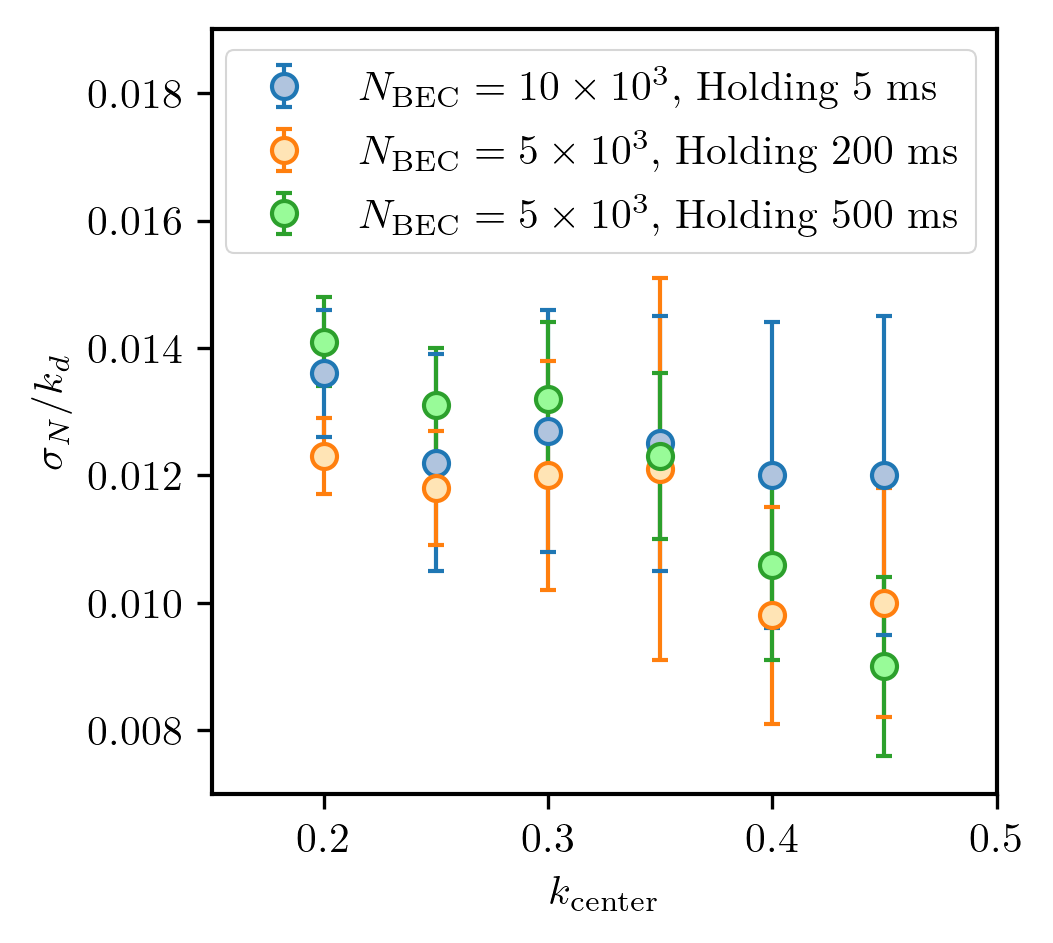
\includegraphics[width=0.7\textwidth]{Fig/Chapter4/sigma_N_vs_k.png}
    \caption[Evolution of the normal correlation peak width $\sigma_N$ with $k$]{Normal correlation peak width $\sigma_N$ as a function of $k_{\rm{center}}$ for various data sets at different temperatures.}
    \label{fig:sigma_N_vs_k}
\end{figure}

As mentioned in the introduction to this section, the results presented here are still quite preliminary and there are quite a few points that need further investigation, notably why the number of detected pair is lower than expected, constituting an interesting prospect for the near future.

\section{Conclusion}

We have reached the end of our investigation of two-body correlation in the depletion of weakly interacting Bose gases. To sum things up, let us remind the main steps of the work conducted during this thesis and its main results.

\begin{itemize}
    \item We decided to try to detect experimentally the \kmk pairs of the quantum depletion predicted by the Bogoliubov theory of the weakly-interacting Bose gas, as this phenomenon is one of the conceptually simplest non-trivial, many-body, quantum correlation effect. By conducting this study, we hope to better understand the physics of many-body equilibrium states and how correlations and entanglement emerge through the combined effects of interactions and quantum fluctuations.
    \item We based our experimental procedure on an experimental setup producing $\He$ BECs  implementing a 3D single-atom resolved electronic detection technique. We decided to use an optical lattice to enter the low-temperature regime dominated by interactions to ensure a sufficient level of quantum depletion so that the \kmk pairs can be properly detected.
    \item We completed previous benchmarking measurements \cite{cayla2018single} by measuring two-body time-of-flight collisions with large number of atoms in the lattice. From this, we were able to conclude that two-body collisions are negligible for the typical number of atoms used in our correlation measurement experiments. This validates the ballistic relation linking the momentum of the in-trap to their detected position after the TOF.
    \item We measured the temperature of the gas at different amplitudes of the lattice potential to certify the adiabatic preparation of the system.
    \item We implemented a two-photon Raman transfer scheme to replace the previous RF transfer, improving the detection efficiency by a factor 2.
    \item We adapted an existing algorithm to make it suited to extract the \kmk correlation signal from the experimental data and benchmarked it with collision spheres data.
    \item We were able to successfully observe anomalous and normal correlation signals in various data sets with different total atom numbers. We validated that the observed anomalous correlation signal is linked to the \kmk pairs of the quantum depletion by observing that:
    \begin{itemize}
        
        \item The signal is lost with temperature, contrary to the normal correlation signal that reveal the chaotic statistics of the system, unaffected by temperature.
        \item The width of the anomalous correlation peak matches the numerical calculations of \cite{butera2020} when accounting for center-of-mass fluctuations.
        \item $\gtwo_A(\bm{0})$ scales linearly with the inverse average momentum density $\bar{\rho}_{\Omega_k}$, while $\gtwo_N(\bm{0})$ remains constant.
        \item We get relative number squeezing between correlated boxes at opposite momenta.
        \item We violate Cauchy-Schwarz inequality by observing $\gtwo_A(\bm{0}) \gg \gtwo_N(\bm{0})$.
        
    \end{itemize}
\end{itemize}

This experimental observations are an encouraging first step towards more ambitious correlation measurements. One of our short term objective is to study the Mott transition and look for complex correlation patterns involving several particles not predicted by simple theoretical treatment such as Bogoliubov theory. As there is currently no theory describing this kind of physics, this represents quite a fascinating prospect that would really put our experiment in the field of quantum simulation. In addition, a more long term prospect would be to improve our experimental setup to bring the fermionic isotope $^3 \mathrm{He}^*$ to quantum degeneracy to perform momentum correlations measurements with fermions and study BEC-BCS crossover physics. A notably important result would be to observe the \kmk pairing of a Cooper pair \cite{cooper1956bound}. Observing the \kmk pairing of the quantum depletion shows us that we are indeed capable of seeing \kmk pairing with our experiment and constitutes a small step towards this result.


